\باب{ترتیب اور تسلسل}
اس باب میں مخلوط اور حقیقی ترتیب اور تسلسل کے بنیادی تصورات پیش کیے جائیں گے۔

\حصہ{ترتیب}\شناخت{حصہ_ترتیب_ترتیب}
تسلسل، بالخصوص طاقتی تسلسل مخلوط تجزیہ میں کلیدی کردار ادا کرتے ہیں۔ان کو متعارف کرنے کی خاطر ہم پہلے ترتیب اور اس سے متعلقہ تصورات کی تعریف پیش کرتے ہیں۔ہم دیکھیں گے کہ مخلوط  ترتیب اور تسلسل کی زیادہ تر مسئلے اور تعریف، حقیقی ترتیب اور تسلسل کے مسائل اور تعریف کی مانند ہوں گے جنہیں حقیقی علم الاحصاء میں استعمال کیا جاتا ہے۔

اگر ہر مثبت عدد صحیح \عددی{n} کو عدد \عددی{z_n} مختص کی جائے تب  ہم کہتے ہیں کہ اعداد
\begin{align*}
z_1,\,z_2,\cdots,z_n,\cdots
\end{align*} 
\اصطلاح{لامتناہی ترتیب}\فرہنگ{ترتیب!لامتناہی}\حاشیہب{infinite sequence}\فرہنگ{sequence} یا،  مختصراً، \اصطلاح{ترتیب} بناتے ہیں۔ان  اعداد \عددی{z_n} کو ترتیب کے \اصطلاح{مقدار} یا  \اصطلاح{اجزاء}\فرہنگ{اجزاء}\حاشیہب{terms}\فرہنگ{terms} کہتے ہیں۔

حقیقی اجزاء پر مبنی ترتیب کو \اصطلاح{حقیقی ترتیب}\فرہنگ{ترتیب!حقیقی}\فرہنگ{حقیقی!ترتیب}\حاشیہب{real sequence}\فرہنگ{real!sequence}\فرہنگ{sequence!real} کہتے ہیں۔

بعض اوقات ہم ترتیب کے اجزاء کی گنتی \عددی{0} یا \عددی{2} یا کسی دیگر عدد صحیح سے شروع کرتے ہیں۔

ایک ترتیب \عددی{z_1,z_2,\cdots} اس صورت \ترچھا{مرکوز}\فرہنگ{مرکوز}  یا \ترچھا{مرتکز}\فرہنگ{مرتکز} ہو گا جب ایسا عدد \عددی{c} پایا جاتا ہو کہ کسی بھی مثبت  (غیر صفر) حقیقی عدد \عددی{\epsilon} (جو چاہے جتنا چھوٹا کیوں نہ ہو) کی صورت میں ہم ایسا عدد صحیح \عددی{N} تلاش کر سکتے ہوں کہ  تمام \عددی{n>N} کے لئے درج ذیل درست ہو۔
\begin{align}\label{مساوات_ترتیب_حد_الف}
\abs{z_n-c}<\epsilon \quad \quad  n>N
\end{align}
\عددی{c} کو ترتیب کا \اصطلاح{حد}\فرہنگ{حد}\حاشیہب{limit}\فرہنگ{limit} کہتے ہیں جس کو عموماً
\begin{align*}
z_n\to c\quad\quad (n\to \infty)
\end{align*}
لکھا جاتا ہے اور ہم کہتے ہیں کہ ترتیب \عددی{c} کو مرکوز ہے یا کہ ترتیب کی حد \عددی{c} ہے۔

ایسی ترتیب جو مرتکز نہ ہو \اصطلاح{منفرج}\فرہنگ{منفرج}\حاشیہب{divergent}\فرہنگ{divergent} کہلاتی ہے۔

مساوات \حوالہ{مساوات_ترتیب_حد_الف} کا  ایک سادہ جیومیٹریائی مطلب ہے۔یہ مساوات کہتی ہے  کہ \عددی{n>N} کی صورت میں ہر جزو \عددی{z_n} اس کھلے قرص میں پایا جاتا ہے جس کا رداس \عددی{\epsilon} اور مرکز \عددی{c} ہے (شکل \حوالہ{شکل_ترتیب_مخلوط_مرتکز})  جبکہ قرص کا رداس \عددی{\epsilon} کتنا ہی کم کیوں نہ کر دیا جائے  اس قرص کے باہر  اجزاء \عددی{z_n} کی زیادہ سے زیادہ تعداد محدود ہو گی۔ظاہر ہے کہ \عددی{N} کی قیمت عموماً \عددی{\epsilon} پر منحصر ہو گی۔
\begin{figure}
\centering
\begin{tikzpicture}
%\draw[thick] (0,0) grid (3,2);
%\draw[thin,gray,step=0.1](0,0) grid (3,2);
%
\draw(0,0)--(3,0)node[right]{$x$};
\draw(0,0)--(0,2)node[left]{$y$};
\foreach \x/\y in {0.1/2,0.2/1.9,0.4/1.8}{\draw[fill](\x,\y)circle (1pt);}
\foreach \x/\y in {0.55/1.85,0.7/1.7,0.9/1.5,1/1.5}{\draw[fill](\x,\y)circle (1pt);}
\foreach \x/\y in {1.05/1.45,1.2/1.35,1.3/1.3,1.3/1.2,1.35/1.2,1.4/1.2}{\draw[fill](\x,\y)circle (1pt);}
\foreach \x/\y in {1.4/1.15,1.5/1.05,1.45/1.15,1.5/1.1}{\draw[fill](\x,\y)circle (1pt);}
\draw(1.5,1)circle (0.75);
\draw[-latex](1.5,1)node[ocirc]{}node[below]{$c$}--++(30:0.75)node[pos=0.35,above]{$\epsilon$};
\end{tikzpicture}
\caption{مرتکز مخلوط ترتیب}
\label{شکل_ترتیب_مخلوط_مرتکز}
\end{figure} 

حقیقی ترتیب کی صورت میں مساوات \حوالہ{مساوات_ترتیب_حد_الف} جیومیٹریائی طور کہتی ہے کہ \عددی{n>N} کی صورت میں جزو \عددی{z_n} وقفہ \عددی{c-\epsilon} تا \عددی{c+\epsilon} پر پایا جائے گا (شکل \حوالہ{شکل_ترتیب_حقیقی_مرتکز}) اور اس وقفہ سے باہر اجزاء کی زیادہ سے زیادہ تعداد محدود ہو گی۔ 
\begin{figure}
\centering
\begin{tikzpicture}
\draw(-2.5,0)--(2.5,0)node[right]{$x$};
\draw(-1.5,0)node[below]{$c-\epsilon$}--++(0,0.1);
\draw(0,0)node[below]{$c$}--++(0,0.1);
\draw(1.5,0)node[below]{$c+\epsilon$}--++(0,0.1);
\end{tikzpicture}
\caption{حقیقی مرتکز ترتیب}
\label{شکل_ترتیب_حقیقی_مرتکز}
\end{figure}

%=======================
\ابتدا{مثال}\شناخت{مثال_ترتیب_مرتکز_اور_منفرج_ترتیب}\quad \موٹا{مرتکز اور منفرج ترتیب}\\
ترتیب \عددی{z_n=1+\tfrac{2}{n}} کے اجزاء 
$3,2,\tfrac{5}{3},\tfrac{6}{4},\tfrac{7}{5},\cdots$
ہیں۔یہ ترتیب  مرتکز ہے اور اس کی حد \عددی{c=1} ہے۔در حقیقت مساوات \حوالہ{مساوات_ترتیب_حد_الف} سے
\begin{align*}
z_n-c=1+\tfrac{2}{n}-1=\tfrac{2}{n}
\end{align*}
لکھا جا سکتا ہے۔یوں \عددی{\tfrac{2}{n}<\epsilon} اس صورت ہو گا جب \عددی{\tfrac{n}{2}>\tfrac{1}{\epsilon}} یا \عددی{n>\tfrac{2}{\epsilon}} ہو۔مثلاً \عددی{\epsilon=0.01} منتخب کرتے ہوئے \عددی{\tfrac{2}{n}<0.01} تب ہو گا جب \عددی{n>200} ہو۔

ترتیب
$1,2,3,\cdots$
اور
$\tfrac{1}{4},\tfrac{3}{4},\tfrac{1}{5},\tfrac{4}{5},\tfrac{1}{6},\tfrac{5}{6},\cdots$
منفرج ہیں۔

وہ ترتیب جس کے اجزاء 
\begin{align*}
z_n=2-\frac{1}{n}+i\big(1+\frac{2}{n}\big)
\end{align*}
یعنی
\begin{align*}
1+i,\quad \frac{3}{2}+i2,\quad \frac{7}{4}+i\frac{3}{2},\cdots
\end{align*}
ہیں کو شکل \حوالہ{شکل_مثال_ترتیب_مرتکز_اور_منفرج_ترتیب} میں دکھایا گیا ہے جہاں پہلے دو اجزاء \عددی{z_1=1+i3} اور \عددی{z_2=\tfrac{3}{2}+i2} کی نشاندہی  کی گئی ہے۔یہ ترتیب مرتکز ہے اور اس کی حد \عددی{c=2+i} ہے۔مساوات \حوالہ{مساوات_ترتیب_حد_الف} سے
\begin{align*}
\abs{z_n-c}=\abs{\frac{2n-1}{n}+i\frac{n+2}{n}-(2+i)}=\abs{-\frac{1}{n}+i\frac{2}{n}}=\frac{\sqrt{5}}{n}
\end{align*}
لکھا جا سکتا ہے۔یوں \عددی{\tfrac{\sqrt{5}}{n}<\epsilon} تب ہو گا جب \عددی{\tfrac{n}{\sqrt{5}}>\tfrac{1}{\epsilon}} یعنی \عددی{n>\tfrac{\sqrt{5}}{\epsilon}} ہو۔مثال کے طور پر \عددی{\epsilon=\tfrac{1}{100}} منتخب کرتے ہوئے  \عددی{\abs{z_n-c}<\epsilon} تب ہو گا جب \عددی{n>223.6} یعنی
\عددی{n=224} یا \عددی{n=225}، وغیرہ ہو۔
\begin{figure}
\centering
\begin{tikzpicture}
\draw(0,0)--(3,0)node[right]{$x$};
\draw(0,0)--(0,3.5)node[right]{$y$};
\foreach \x in {1,2}{\draw(\x,0)node[below]{$\x$}--++(0,0.1);}
\foreach \y in {1,2,3}{\draw(0,\y)node[left]{$\y$}--++(0.1,0);}
\foreach \n in {1,2,3,4,5,6,7,8,9,10,11,12,16,20,25,30,40,60,80,90,100}{\draw[fill](2-1/\n,1+2/\n) circle (1pt);}
\draw(2,1)node[ocirc]{}node[right]{$c=2+i$};
\draw(0,0)node[below]{$0$}node[left]{$0$};
\draw(1,3)node[right]{$z_1$};
\draw(3/2,2)node[right]{$z_2$};
\end{tikzpicture}
\caption{مثال \حوالہ{مثال_ترتیب_مرتکز_اور_منفرج_ترتیب} میں آخری ترتیب}
\label{شکل_مثال_ترتیب_مرتکز_اور_منفرج_ترتیب}
\end{figure}
\انتہا{مثال}
%===========================
مخلوط ترتیب \عددی{z_1,z_2,z_3,\cdots} کی صورت میں \عددی{z_n=x_n+iy_n} لکھ کر ہم حقیقی حصوں کی ترتیب اور خیالی حصوں کی ترتیب
\begin{align*}
x_1,x_2,x_3,\cdots\quad \text{اور}\quad y_1,y_2,y_3,\cdots
\end{align*}
 پر علیحدہ علیحدہ غور کر سکتے ہیں۔مثلاً  مثال \حوالہ{مثال_ترتیب_مرتکز_اور_منفرج_ترتیب} کی آخری ترتیب کے دو علیحدہ علیحدہ ترتیب درج ذیل ہوں گی۔
\begin{align*}
1,\frac{3}{2},\frac{5}{3},\frac{7}{4},\cdots \quad \text{اور}\quad 3,2,\frac{5}{3},\frac{3}{2},\cdots
\end{align*}
ہم دیکھتے ہیں کہ حقیقی اور خیالی ترتیب کے حد  بالترتیب \عددی{2} اور \عددی{1} ہیں (شکل \حوالہ{شکل_مثال_ترتیب_مرتکز_اور_منفرج_ترتیب}) جو اصل مخلوط ترتیب کی حقیقی اور خیالی حصوں کی حد ہیں۔عموماً ایسا ہی ہوتا ہے جو درج ذیل کی ایک مثال ہے۔ 

%==================
\ابتدا{مسئلہ}\شناخت{مسئلہ_ترتیب_حقیقی_خیالی_اجزاء_ترتیب}\quad \موٹا{(حقیقی اور خیالی اجزاء کی ترتیب)}\\
مخلوط اعداد \عددی{z_n=x_n+iy_n\quad (n=1,2,\cdots)} کی ترتیب \عددی{z_1,z_2,\cdots,z_n,\cdots} صرف اور صرف اس صورت حد \عددی{c=a+ib} پر مرکوز ہو گا جب حقیقی حصوں کی ترتیب   \عددی{x_1,x_2,\cdots} نقطہ \عددی{a} پر مرتکز ہو اور خیالی حصوں کی ترتیب \عددی{y_1,y_2,\cdots} نقطہ \عددی{b} پر مرتکز ہو۔
\انتہا{مسئلہ}
%=======================
\ابتدا{ثبوت}\quad
اگر \عددی{\abs{z_n-c}<\epsilon} ہو تب  \عددی{z_n=x_n+iy_n} اس دائرہ کے اندر پایا جائے گا جس کا رداس \عددی{\epsilon} اور مرکز \عددی{c=a+ib} ہوں۔ یوں لازماً 
\begin{align*}
\abs{x_n-a}<\epsilon, \quad \abs{y_n-b}<\epsilon
\end{align*}
ہو گا (شکل \حوالہ{شکل_مسئلہ_ترتیب_حقیقی_خیالی_اجزاء_ترتیب}-الف)۔ یوں \عددی{n\to \infty} کی صورت میں مرکوزیت \عددی{z_n\to c} سے مراد مرکوزیت \عددی{x_n\to a} اور مرکوزیت \عددی{y_n\to b} ہے۔
\begin{figure}
\centering
\begin{subfigure}{0.5\textwidth}
\centering
\begin{tikzpicture}
\pgfmathsetmacro{\xlen}{1.5}
\pgfmathsetmacro{\ylen}{1.5}
\pgfmathsetmacro{\r}{1}
\draw(\xlen,\ylen)coordinate(kA);
%
\draw(0,0)--(3.5,0)node[right]{$x$};
\draw(0,0)--(0,3)node[right]{$y$};
%
\draw[dashed](kA)--(\xlen,0)node[below]{$a$};
\draw[dashed](kA)--(0,\ylen)node[left]{$b$};
\draw[dashed](\xlen,\ylen+\r)--(0,\ylen+\r)node[left]{$b+\epsilon$};
\draw[dashed](\xlen,\ylen-\r)--(0,\ylen-\r)node[left]{$b-\epsilon$};
\draw[dashed](\xlen-\r,\ylen)--(\xlen-\r,0)node[below]{$a-\epsilon$};
\draw[dashed](\xlen+\r,\ylen)--(\xlen+\r,0)node[below]{$a+\epsilon$};
\draw(kA)node[ocirc]{}node[right]{$c$} circle (\r);
\end{tikzpicture}
\caption*{(الف)}
\end{subfigure}%
\begin{subfigure}{0.5\textwidth}
\centering
\begin{tikzpicture}
\pgfmathsetmacro{\xlen}{1.5}
\pgfmathsetmacro{\ylen}{1.5}
\pgfmathsetmacro{\r}{1}
\draw(\xlen,\ylen)coordinate(kA);
%
\draw(0,0)--(3.5,0)node[right]{$x$};
\draw(0,0)--(0,3)node[right]{$y$};
%
\draw[dashed](kA)--(\xlen,0)node[below]{$a$};
\draw[dashed](kA)--(0,\ylen)node[left]{$b$};
\draw[dashed](\xlen-\r/2,\ylen+\r/2)--(0,\ylen+\r/2)node[left]{$b+\tfrac{\epsilon}{2}$};
\draw[dashed](\xlen-\r/2,\ylen-\r/2)--(0,\ylen-\r/2)node[left]{$b-\tfrac{\epsilon}{2}$};
\draw[dashed](\xlen-\r/2,\ylen-\r/2)--(\xlen-\r/2,0);
\draw[dashed](\xlen+\r/2,\ylen-\r/2)--(\xlen+\r/2,0);
\draw(kA)node[ocirc]{}node[right]{$c$} circle (\r);
\draw[thick](\xlen-\r/2,\ylen-\r/2) rectangle ++(\r,\r);
\draw[stealth-](\xlen-\r/2,0)++(0,-0.1) to [out=-90,in=0]++(-0.3,-0.3)node[left]{$a-\tfrac{\epsilon}{2}$};
\draw[stealth-](\xlen+\r/2,0)++(0,-0.1) to [out=-90,in=180]++(0.3,-0.3)node[right]{$a+\tfrac{\epsilon}{2}$};
\end{tikzpicture}
\caption*{(ب)}
\end{subfigure}%
\caption{مسئلہ \حوالہ{مسئلہ_ترتیب_حقیقی_خیالی_اجزاء_ترتیب} کا ثبوت}
\label{شکل_مسئلہ_ترتیب_حقیقی_خیالی_اجزاء_ترتیب}
\end{figure}

اس کی الٹ چلتے ہوئے، اگر \عددی{n\to \infty} کی صورت میں \عددی{x_n\to a} اور \عددی{y_n\to b} ہوں  تب کسی بھی دیے گئے \عددی{\epsilon>0} کی صورت میں ہم ایسا \عددی{N} اتنا بڑا منتخب کر سکتے ہیں کہ ہر \عددی{n>N} کے لئے 
\begin{align*}
\abs{x_n-a}<\frac{\epsilon}{2},\quad \abs{y_n-b}<\frac{\epsilon}{2}
\end{align*}
ہو۔ان دو عدم مساوات کہتی ہیں کہ \عددی{z_n=x_n+iy_n} اس چکور کے اندر پایا جائے گا جس کے اطراف کی لمبائی \عددی{\epsilon} اور مرکز \عددی{c} ہو (شکل \حوالہ{شکل_مسئلہ_ترتیب_حقیقی_خیالی_اجزاء_ترتیب}-ب)۔یوں ثبوت مکمل ہوتا ہے۔
\انتہا{ثبوت}
%=================

اس مسئلہ کی باعث حقیقی حصہ اور خیالی حصہ کی ترتیب پر غور کرتے ہوئے مخلوط ترتیب کی مرکوزیت کو حقیقی ترتیب سے حاصل کیا جا سکتا ہے۔

اگر ایسا مثبت عدد \عددی{K} پایا جاتا ہو کہ مرکز پر رداس \عددی{K} کے دائرے میں ترتیب \عددی{z_1,z_2,\cdots} کے تمام اجزاء  پائے جاتے ہوں  یعنی
\begin{align*}
\abs{z_n}<K \quad \quad \text{\RL{تمام $n$}}
\end{align*}
تب یہ ترتیب \اصطلاح{محدود}\فرہنگ{محدود}\حاشیہب{bounded}\فرہنگ{bounded} کہلاتا  ہے۔ایسی ترتیب جو محدود نہ ہو \اصطلاح{غیر محدود}\فرہنگ{غیر محدود}\حاشیہب{unbounded}\فرہنگ{unbounded} کہلاتا ہے۔

اس تصور کو استعمال کرتے ہوئے انفراج  کو عموماً درج ذیل سادہ مسئلہ  سے دریافت کیا جا سکتا ہے۔

%=========================
\ابتدا{مسئلہ}\شناخت{مسئلہ_ترتیب_مرتکز_ترتیب_محدود_ہو_گی}
ہر مرتکز ترتیب محدود ہو گی۔یوں اگر ایک ترتیب غیر محدود ہو تب یہ منفرج ہو گی۔
\انتہا{مسئلہ}
%===========================
\ابتدا{ثبوت}
فرض کریں کہ ترتیب \عددی{z_1,z_2,\cdots} مرکوز ہے اور اس کی حد \عددی{c} ہے۔ تب ہم \عددی{\epsilon>0} منتخب کرتے ہوئے ایسا مطابقتی \عددی{N} تلاش کر سکتے ہیں کہ  \عددی{n>N} کے لئے ہر \عددی{z_n} رداس \عددی{\epsilon} کے قرص، جس کا مرکز \عددی{c} ہو، میں پائے جائیں گے اور وہ  \عددی{z_n} جو اس قرص کے باہر ہوں کی زیادہ سے زیادہ تعداد محدود ہو گی۔اب ظاہر ہے کہ ہم مرکز پر اتنے بڑی  رداس \عددی{K} کا دائرہ منتخب کر سکتے ہیں کہ یہ قرص اور قرص کے باہر تمام \عددی{z_n} اس دائرے میں پائیں جاتے ہوں۔اس سے ثابت ہوتا ہے کہ یہ ترتیب محدود ہے۔
\انتہا{ثبوت}
%=========================

یہاں دہان رہے کہ محدود ہونا مرکوزیت کے لئے کافی نہیں ہے۔مثلاً ترتیب \عددی{1,0,1,0,\cdots} محدود  لیکن منفرج ہے۔ (کیوں؟) غیر محدود ترتیب کی مثالیں درج ذیل ہیں
\begin{align*}
1,2,3,4,\cdots\quad \text{اور}\quad \frac{1}{2},2,\frac{1}{3},3,\frac{1}{4},4,\cdots
\end{align*} 
جو مسئلہ \حوالہ{مسئلہ_ترتیب_مرتکز_ترتیب_محدود_ہو_گی} کے تحت منفرج ترتیب ہیں۔

%=====================
\حصہء{سوالات}
سوال \حوالہ{سوال_ترتیب_نقشہ_الف} تا سوال \حوالہ{سوال_ترتیب_نقشہ_ب} میں دیے ترتیب کے ابتدائی چند اجزاء لکھ کر ترسیم کریں۔

%======================
\ابتدا{سوال}\شناخت{سوال_ترتیب_نقشہ_الف}\quad
$\tfrac{n}{n+3}$\\
جواب:\quad
$\tfrac{1}{4},\tfrac{2}{5},\tfrac{1}{2},\tfrac{4}{7},\tfrac{5}{8},\cdots$
\انتہا{سوال}
%======================
\ابتدا{سوال}\quad
$\tfrac{2n}{n^2+1}$\\
جواب:\quad
$1,\tfrac{4}{5},\tfrac{3}{5},\tfrac{8}{17},\tfrac{5}{13},\cdots$
\انتہا{سوال}
%======================
\ابتدا{سوال}\شناخت{سوال_ترتیب_نقشہ_پ}\quad
$\tfrac{i^n}{n^2}$\\
جواب:\quad
$i,-\tfrac{1}{4},-\tfrac{i}{9},\tfrac{1}{16},\tfrac{i}{25},\cdots$
\انتہا{سوال}
%======================
\ابتدا{سوال}\quad
$\tfrac{in}{n+1}$\\
جواب:\quad
$\tfrac{i}{2},\tfrac{i2}{3},\tfrac{i3}{4},\tfrac{i4}{5},\tfrac{i5}{6},\cdots$
\انتہا{سوال}
%======================
\ابتدا{سوال}\quad
$\tfrac{i^n n^2}{n+i}$\\
جواب:\quad
$\tfrac{1}{2}(1+i),\tfrac{4}{5}(-2+i),\tfrac{9}{10}(-1-i3),\tfrac{16}{17}(4-i),\tfrac{25}{26}(1+i5),\cdots$
\انتہا{سوال}
%======================
\ابتدا{سوال}\شناخت{سوال_ترتیب_نقشہ_ب}\quad
$(-1)^n+i2\pi n$\\
جواب:\quad
$-1+i2\pi, 1+i4\pi,-1+i6\pi, 1+i8\pi, -1+i10\pi,\cdots$
\انتہا{سوال}
%======================
\ابتدا{سوال}\quad
ترتیب \عددی{z_1=1}، \عددی{z_2=\tfrac{i}{2}}، \عددی{z_n=iz_{n-2}z_{n-1}\,\, (n=3,4,\cdots)} کے ابتدائی چند اجزاء لکھیں۔اس ترتیب  کی حد تلاش کریں۔\\
جواب:\quad
$1,\tfrac{i}{2}, -\tfrac{1}{2},\tfrac{1}{4}, -\tfrac{i}{8},\cdots$
\انتہا{سوال}
%=========================
سوال \حوالہ{سوال_ترتیب_محدود_مرکوز_حد_الف} تا سوال \حوالہ{سوال_ترتیب_محدود_مرکوز_حد_ب} میں دریافت کریں کہ آیا دی گئی ترتیب محدود ہے؟ کیا یہ ترتیب مرکوز ہے؟ مرکوزیت کی صورت میں ترتیب کی حد تلاش کریں۔
  
%================
\ابتدا{سوال}\شناخت{سوال_ترتیب_محدود_مرکوز_حد_الف}\quad
$z_n=i^n$\\
جواب:\quad
محدود، منفرج
\انتہا{سوال}
%======================
\ابتدا{سوال}\quad
$z_n=\tfrac{i^n}{n}$\\
جواب:\quad
محدود، مرکوز، حد $0$
\انتہا{سوال}
%======================
\ابتدا{سوال}\quad
$z_n=\tfrac{in}{n+1}$\\
جواب:\quad
محدود، مرکوز، حد $i$
\انتہا{سوال}
%======================
\ابتدا{سوال}\quad
$z_n=\tfrac{n^2}{n+i}$\\
جواب:\quad
غیر محدود، منفرج
\انتہا{سوال}
%======================
\ابتدا{سوال}\quad
$z_n=\tfrac{(-1)^n}{n^3}$\\
جواب:\quad
محدود، مرکوز، حد $0$
\انتہا{سوال}
%======================
\ابتدا{سوال}\شناخت{سوال_ترتیب_محدود_مرکوز_حد_ب}\quad
$z_n=e^{i\tfrac{n\pi}{4}}$\\
جواب:\quad
محدود، منفرج
\انتہا{سوال}
%======================
\ابتدا{سوال}\quad \موٹا{حد کی یکتائی}\\
دکھائیں کہ اگر ایک ترتیب مرتکز ہو تب اس کا حد یکتا ہو گا۔
\انتہا{سوال}
%=========================
\ابتدا{سوال}\quad
ثابت کریں (مثال \حوالہ{مثال_ترتیب_مرتکز_اور_منفرج_ترتیب} کی طرح) کہ 
$\tfrac{i^n}{n^3}$
مرکوز ہے۔
\انتہا{سوال}
%============================
\ابتدا{سوال}\quad
ایک ترتیب کے اجزاء درج ذیل کلیہ دیتی ہے۔اس ترتیب کو استعمال کرتے ہوئے مسئلہ \حوالہ{مسئلہ_ترتیب_حقیقی_خیالی_اجزاء_ترتیب} کی تصدیق کریں۔\\
\begin{align*}
z_n=\frac{n^2-1}{2n^2+1}+i\frac{n}{n+2}
\end{align*}
\انتہا{سوال}
%====================
\ابتدا{سوال}\quad
دکھائیں کہ مخلوط ترتیب \عددی{z_1,z_2,\cdots} اس صورت محدود ہو گی جب اس کے حقیقی حصہ اور خیالی حصہ کے مطابقتی ترتیب محدود ہوں۔
\انتہا{سوال}
%====================
\ابتدا{سوال}\quad
اگر ترتیب \عددی{z_1,z_2,\cdots} مرکوز ہو اور اس کا حد \عددی{0} ہو، اور ترتیب \عددی{b_1,b_2,\cdots} کسی مقررہ \عددی{K>0} اور تمام \عددی{n} کے  لئے  \عددی{\abs{b_n}\le K\abs{z_n}} کو مطمئن کرتا ہو تب دکھائیں کہ ترتیب \عددی{b_1,b_2,\cdots} مرکوز ہے اور اس کا حد \عددی{0} ہے۔
\انتہا{سوال}
%========================
\ابتدا{سوال}\شناخت{سوال_ترتیب_مجموعہ_کا_حد}\quad
اگر ترتیب \عددی{z_1,z_2,\cdots} مرکوز ہو اور اس کا حد \عددی{l} ہو اور ترتیب \عددی{z^*_1,z^*_2,\cdots} مرکوز ہو اور اس کا حد \عددی{l^*}  ہو تب دکھائیں کہ ترتیب \عددی{z_1+z^*_1,z_2+z^*_2,\cdots} مرکوز ہو گا اور اس کا حد \عددی{l+l^*} ہو گا۔
\انتہا{سوال}
%=========================
\ابتدا{سوال}\quad
سوال \حوالہ{سوال_ترتیب_مجموعہ_کا_حد} کے مفروضوں کے ساتھ دکھائیں کہ ترتیب \عددی{z_1z^*_1,z_2z^*_2,\cdots}  مرکوز ہو گا اور اس کا حد \عددی{ll^*} ہو گا۔
\انتہا{سوال}
%========================

\حصہ{تسلسل}\شناخت{حصہ_ترتیب-تسلسل}
فرض کریں کہ \عددی{w_1,w_2,\cdots,w_m,\cdots} حقیقی یا مخلوط اعداد کی ترتیب ہے۔تب ہم درج ذیل \ترچھا{لامتناہی تسلسل} یا، مختصراً، \اصطلاح{تسلسل}\فرہنگ{تسلسل}\حاشیہب{series}\فرہنگ{series} پر غور کرتے ہیں۔
\begin{align}\label{مساوات_ترتیب_تسلسل_الف}
\sum_{m=1}^{\infty} w_m=w_1+w_2+w_3+\cdots
\end{align}
\عددی{w_m} کو ترتیب کی \ترچھا{مقدار} یا  \اصطلاح{اجزاء}\فرہنگ{اجزاء}\حاشیہب{terms}\فرہنگ{terms} کہتے ہیں۔ابتدائی \عددی{n} اجزاء کے مجموعہ
\begin{align}\label{مساوات_ترتیب_تسلسل_ب}
s_n=w_1+w_2+\cdots+w_n
\end{align}
کو تسلسل \حوالہ{مساوات_ترتیب_تسلسل_الف} کا \عددی{n} واں \اصطلاح{جزوی مجموعہ}\فرہنگ{جزوی مجموعہ}\فرہنگ{مجموعہ!جزوی}\حاشیہب{partial sum}\فرہنگ{sum!partial} کہتے ہیں۔ تسلسل \حوالہ{مساوات_ترتیب_تسلسل_الف} سے  \عددی{s_n} ترک کرنے سے
\begin{align}
R_n=w_{n+1}+w_{n+2}+w_{n+3}+\cdots
\end{align}
باقی رہ جاتا ہے جس کو تسلسل \حوالہ{مساوات_ترتیب_تسلسل_الف} کا، \عددی{n} اجزاء کے بعد، \اصطلاح{باقی}\فرہنگ{باقی}\حاشیہب{remainder}\فرہنگ{remainder} کہتے ہیں۔ 

اس طرح ہم تسلسل \حوالہ{مساوات_ترتیب_تسلسل_الف} کے ساتھ اس کے جزوی مجموعوں \عددی{s_1,s_2,s_3,\cdots} کی ترتیب وابستہ کرتے ہیں۔اگر یہ ترتیب مرتکز ہو، مثلاً،
\begin{align*}
\lim_{n\to \infty} s_n=s
\end{align*}
تب ہم کہتے ہیں کہ تسلسل \حوالہ{مساوات_ترتیب_تسلسل_الف} \اصطلاح{مرکوز}\فرہنگ{مرکوز}\حاشیہب{convergent}\فرہنگ{convergent} یا \اصطلاح{مرتکز} ہے اور عدد \عددی{s} اس کی \اصطلاح{قیمت}\فرہنگ{قیمت}\حاشیہب{value}\فرہنگ{value} یا \ترچھا{مجموعہ}\فرہنگ{مجموعہ} کہلاتا ہے اور ہم درج ذیل لکھتے ہیں۔
\begin{align*}
s=\sum_{m=1}^{\infty} w_m=w_1+w_2+w_3+\cdots
\end{align*}

اگر جزوی مجموعوں کی ترتیب منفرج ہو تب ہم کہتے ہیں کہ تسلسل  \حوالہ{مساوات_ترتیب_تسلسل_الف}  \اصطلاح{منفرج}\فرہنگ{منفرج}\حاشیہب{divergent}\فرہنگ{divergent} ہے۔

اگر تسلسل \حوالہ{مساوات_ترتیب_تسلسل_الف} مرکوز ہو اور اس کی قیمت \عددی{s} ہو تب
\begin{align}
s=s_n+R_n\quad \implies \quad R_n=s-s_n
\end{align}
ہو گا۔مرکوزیت کی تعریف کے تحت \عددی{n} کو کافی بڑا لیتے ہوئے  ہم \عددی{\abs{R_n}} کو جتنا چاہیں چھوٹا بنا سکتے ہیں۔ بہت سی صورتوں میں مرکوز تسلسل کا مجموعہ \عددی{s} تلاش کرنا نا ممکن ہو گا۔تب حساب کی خاطر ہم اس کے جزوی مجموعہ \عددی{s_n} کو \عددی{s} کی تقریب تصور کریں گے اور \عددی{R_n} کا تخمینہ لگا کر  تقریب کی درستگی کا جائزہ لیں گے۔

%===================
\ابتدا{مثال}\شناخت{مثال_ترتیب_ہارمونی_منفرج}\quad \موٹا{مرتکز اور منفرج تسلسل}\\
تسلسل
\begin{align*}
\sum_{m=1}^{\infty} \frac{1}{2^m}=\frac{1}{2}+\frac{1}{4}+\frac{1}{8}+\cdots
\end{align*}
مرکوز ہے اور چونکہ
\begin{align*}
s_n=\frac{1}{2}+\frac{1}{4}+\frac{1}{8}+\cdots+\frac{1}{2^n}=1-\frac{1}{2^n} \quad \implies\quad  \lim_{n\to \infty}s_n=1
\end{align*}
ہے لہٰذا تسلسل کی قیمت \عددی{1} ہے۔اس کے برعکس تسلسل
\begin{align*}
\sum_{m=1}^{\infty} m=1+2+3+\cdots
\end{align*}
منفرج ہے اور تسلسل
\begin{align*}
\sum_{m=0}^{\infty} (-1)^m=1-1+1-+\cdots
\end{align*}
منفرج ہے چونکہ 
\begin{align*}
s_0=1, \quad s_1=1-1=0,\quad s_2=1-1+1=1, \cdots
\end{align*}
ہے  اور ترتیب \عددی{1,0,1,0,\cdots} منفرج ہے۔

\اصطلاح{ہارمونی تسلسل}\فرہنگ{ہارمونی!تسلسل}\حاشیہب{harmonic series}\فرہنگ{harmonic!series}
\begin{align*}
\sum_{m=1}^{\infty} \frac{1}{m}=1+\frac{1}{2}+\frac{1}{3}+\cdots
\end{align*}
منفرج ہے۔در حقیقت جزوی مجموعہ \عددی{s_n}
\begin{align*}
s_n=1+\frac{1}{2}+\cdots+\frac{1}{n}
\end{align*}
شکل \حوالہ{مثال_ترتیب_ہارمونی_منفرج} میں \عددی{n} عدد مستطیل کے نیچے رقبہ کے برابر ہے۔یہ رقبہ قوس \عددی{y=\tfrac{1}{x}} کے نیچے مطابقتی رقبہ \عددی{A_n} سے زیادہ ہے۔اب 
\begin{align*}
A_n=\int_1^{n+1}\frac{\dif x}{x}=\ln(n+1)\to \infty \quad \quad (n\to \infty)
\end{align*}
ہے اور چونکہ \عددی{s_n>A_n} ہے لہٰذا \عددی{n\to \infty} کرنے سے \عددی{s_n\to\infty} حاصل ہو گا جو انفراج کی تعریف ہے۔
\begin{figure}
\centering
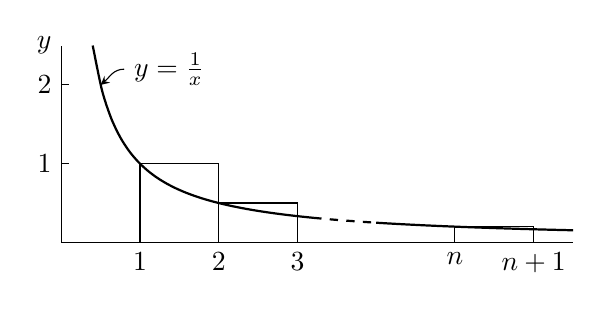
\begin{tikzpicture}
\draw(0,0)--(6.5,0);
\draw(0,0)--(0,2.5)node[left]{$y$};
\foreach \x in {1,2,3}{\draw(\x,0)node[below]{$\x$};}
\foreach \y in {1,2}{\draw(0,\y)node[left]{$\y$}--++(0.1,0);}
\draw[thick,domain=0.4:3.2,variable=\x,smooth]  plot ({\x},{1/\x});
\draw[thick,dashed,domain=3.2:4,variable=\x,smooth]  plot ({\x},{1/\x});
\draw[thick,domain=4:6.5,variable=\x,smooth]  plot ({\x},{1/\x});
\draw(1,0)--++(0,1)--++(1,0)--++(0,-1);
\draw(2,1/2)--++(1,0)--++(0,-1/2);
\draw(5,0)node[below]{$n$}--++(0,0.2)--++(1,0)--++(0,-0.2)node[below]{$n+1$};
\draw[stealth-](0.5,2) to [out=40,in=180]++(0.3,0.2)node[right]{$y=\frac{1}{x}$};
\end{tikzpicture}
\caption{شکل برائے مثال \حوالہ{مثال_ترتیب_ہارمونی_منفرج}}
\label{شکل_مثال_ترتیب_ہارمونی_منفرج}
\end{figure}
\انتہا{مثال}
%========================

مسئلہ \حوالہ{مسئلہ_ترتیب_حقیقی_خیالی_اجزاء_ترتیب} سے  فوری طور پر تسلسل کے لئے درج ذیل مسئلہ حاصل ہوتا ہے۔

%===============
\ابتدا{مسئلہ}\quad \موٹا{حقیقی اور خیالی حصوں کی تسلسل}\\
فرض کریں کہ \عددی{w_m=u_m+iv_m} ہے۔تب تسلسل
\begin{align*}
\sum_{m=1}^{\infty} w_m=w_1+w_2+w_3+\cdots
\end{align*}
کی قیمت صرف اور صرف اس صورت \عددی{s=a+jb} ہو گی جب حقیقی حصہ کی تسلسل اور خیالی حصہ کی تسلسل 
\begin{align*}
\sum_{m=1}^{\infty} u_m=u_1+u_2+u_3+\cdots\quad \text{}\quad \sum_{m=1}^{\infty} v_m=v_1+v_2+v_3+\cdots
\end{align*}
مرکوز ہوں اور حقیقی حصے کی تسلسل کی قیمت \عددی{a} اور خیالی حصے کی تسلسل کی قیمت  \عددی{b} ہو۔
\انتہا{مسئلہ}
%====================== 

یہ مسئلہ حقیقی اور مخلوط تسلسل کے درمیان تعلق دیتا ہے۔اس سے زیادہ اہم تعلق درج ذیل تصور پر مبنی ہے۔ 

تسلسل \عددی{w_1+w_2+\cdots} اس صورت \اصطلاح{حتمی مرتکز}\فرہنگ{مرتکز!حتمی}\حاشیہب{absolutely convergent}\فرہنگ{convergent!absolutely}  کہلاتا ہے جب مطابقتی تسلسل
\begin{align}\label{مساوات_ترتیب_حتمی_مرتکز}
\sum_{m=1}^{\infty} \abs{w_m}=\abs{w_1}+\abs{w_2}+\cdots
\end{align}
(جس کے اجزاء حقیقی اور غیر منفی ہیں) مرتکز ہو۔

اگر تسلسل \عددی{w_1+w_2+\cdots} مرکوز ہو جبکہ  تسلسل \حوالہ{مساوات_ترتیب_حتمی_مرتکز} منفرج ہو تب تسلسل  \اصطلاح{مشروط مرتکز}\فرہنگ{مرتکز!مشروط}\حاشیہب{conditional convergent}\فرہنگ{convergent!conditional}  کہلاتا ہے۔

%====================
\ابتدا{مثال}\شناخت{مثال_ترتیب_حتمی_اور_مشروط_مرکوز_تسلسل}\quad \موٹا{حتمی اور مشروط مرکوز تسلسل}\\
تسلسل
\begin{align*}
\frac{1}{2}-\frac{1}{4}+\frac{1}{8}-\frac{1}{16}+-\cdots
\end{align*}
حتمی مرتکز ہے چونکہ مطابقتی تسلسل \حوالہ{مساوات_ترتیب_حتمی_مرتکز} مرکوز ہے (مثال \حوالہ{مثال_ترتیب_ہارمونی_منفرج})۔اس کے برعکس تسلسل
\begin{align*}
1-\frac{1}{2}+\frac{1}{3}-\frac{1}{4}+-\cdots
\end{align*}
مشروط مرکوز ہے چونکہ تسلسل از خود  (لیبنٹز آزمائش  کے تحت جس پر حصہ \حوالہ{حصہ_ترتیب_لیبنٹز_آزمائش_برائے_حقیقی_تسلسل} میں غور کیا جائے گا)   مرتکز ہے لیکن مطابقتی تسلسل \حوالہ{مساوات_ترتیب_حتمی_مرتکز} ہارمونی ہے جو منفرج ہے (مثال \حوالہ{مثال_ترتیب_ہارمونی_منفرج})۔
\انتہا{مثال}
%===========================

حتمی مرتکز تسلسل کی درج ذیل خاصیت بالکل واضح ہے۔

%=============== 
\ابتدا{مسئلہ}\شناخت{مسئلہ_ترتیب_حتمی_مرتکز_مرکوز_ہو_گا}
اگر تسلسل \عددی{w_1+w_2+\cdots} حتمی مرتکز ہو تب یہ تسلسل مرتکز ہو گا۔
\انتہا{مسئلہ}
%=======================

ہم اگلے حصے کی آخر میں کوشی اصول مرکوزیت کی مدد سے مسئلہ \حوالہ{مسئلہ_ترتیب_کوشی_اصول_استعمال_الف} میں   اس مسئلے کا سادہ ثبوت پیش کریں گے ۔

ہم آخر میں ایک سادہ مسئلہ پیش کرتے ہیں جو عموماً کارآمد ثابت ہوتا ہے۔

%=====================
\ابتدا{مسئلہ}\شناخت{مسئلہ_ترتیب_مرکوزیت_شرط}\شناخت{مسئلہ_ترتیب_آزمائش_مرکوزیت_حقیقی}
اگر تسلسل \عددی{w_1+w_2+\cdots} مرتکز ہو تب
\begin{align}\label{مساوات_ترتیب_مرکوزیت_شرط}
\lim_{m\to\infty} w_m=0
\end{align}
ہو گا۔یوں وہ تسلسل جو مساوات \حوالہ{مساوات_ترتیب_مرکوزیت_شرط} کو مطمئن نہ کرتا ہو منفرج ہو گا۔
\انتہا{مسئلہ}
%==============================
\ابتدا{ثبوت}\quad
فرض کریں کہ \عددی{w_1+w_2+\cdots} مرتکز ہے اور اس کا مجموعہ \عددی{s} ہے۔ تب 
\begin{align*}
w_{n+1}=s_{n+1}-s_n
\end{align*}
اور
\begin{align*}
\lim_{n\to\infty} (s_{n+1}-s_n)=\lim_{n\to\infty}s_{n+1} -\lim_{n\to\infty}s_n=s-s=0
\end{align*}
ہو گا۔
\انتہا{ثبوت}
%==========================

یاد رہے کہ مساوات \حوالہ{مساوات_ترتیب_مرکوزیت_شرط} مرکوزیت کے لئے لازمی لیکن نا کافی شرط ہے۔ مثلاً مثال \حوالہ{مثال_ترتیب_ہارمونی_منفرج} کی ہارمونی تسلسل مساوات \حوالہ{مساوات_ترتیب_مرکوزیت_شرط} کو مطمئن کرتے ہوئے بھی  منفرج ہے۔  مساوات \حوالہ{مساوات_ترتیب_مرکوزیت_شرط} میں دوسری اور تیسری تسلسل مساوات  \حوالہ{مساوات_ترتیب_مرکوزیت_شرط} کو مطمئن نہیں کرتے ہیں لہٰذا وہ منفرج ہیں۔

%============================
\حصہ{کوشی اصول مرکوزیت برائے ترتیب اور تسلسل}\شناخت{حصہ_ترتیب_کوشی_اصول_مرکوزیت_ترتیب_تسلسل}\فرہنگ{کوشی کا اصول مرکوزیت}\فرہنگ{Cauchy' convergence principle}
کسی بھی ترتیب یا تسلسل کو استعمال کرنے سے پہلے ہم جاننا چاہیں گے کہ آیا وہ مرتکز ہے یا نہیں۔چونکہ ہمیں پہلے سے حد معلوم نہیں ہوتا ہے لہٰذا مرکوزیت کی تعریف سے ایسا فیصلہ کرنا عموماً ممکن نہیں ہو گا۔کوشی اصول مرکوزیت سے، حد جانے بغیر مرکوزیت دریافت کرتا ہے۔

کوشی اصول مرکوزیت میں ہم  مسئلہ بُلزانو وائشسٹراس زیر استعمال لائیں گے۔ مسئلہ بُلزانو وائشسٹراس کو بیان کرنے کی خاطر درج ذیل تصور کی ضرورت ہو گی۔  

نقطہ \عددی{a} اس صورت ترتیب \عددی{z_1,z_2,\cdots} کا \اصطلاح{تحدیدی نقطہ}\فرہنگ{تحدیدی!نقطہ}\فرہنگ{نقطہ!تحدیدی}\حاشیہب{limit point}\فرہنگ{limit!point} کہلائے گا جب کسی بھی دیے گئے \عددی{\epsilon>0} (جو جتنا چاہیں چھوٹا کیوں نا ہو)  کے لئے درج ذیل درست ہو۔
\begin{align}\label{مساوات_ترتیب_تحدیدی_نقطہ}
\abs{z_n-a}<\epsilon \quad \quad \text{\RL{(جہاں \عددی{n} لامتناہی تعداد ہے)}}
\end{align}
جیومیٹریائی طور پر اس کا مطلب ہے کہ \عددی{\epsilon} کو جتنا بھی چھوٹا کیوں نہ منتخب کیا جائے، رداس \عددی{\epsilon} کا دائرہ جس کا مرکز \عددی{a} ہو، میں تسلسل کے نقطوں کی لامتناہی تعداد پائی جائے گی۔

دھیان رہے کہ مساوات \حوالہ{مساوات_ترتیب_تحدیدی_نقطہ} مطمئن ہونے کے باوجود  دائرے کے باہر نقطوں کی تعداد لامتناہی ہو سکتی ہے اور ترتیب منفرج ہو سکتا ہے۔ در حقیقت مرتکز ترتیب کا حد ہی تحدیدی نقطہ ہو گا (کیوں؟)  اور یہ ترتیب کا واحد تحدیدی نقطہ ہو گا۔اگر کسی ترتیب کا ایک سے زیادہ تحدیدی نقطہ پایا جاتا ہو تب یہ ترتیب منفرج ہو گا۔

مزید، اگر ایک نقطہ لامتناہی بار کسی ترتیب میں پایا جاتا ہو تب تحدیدی نقطہ کی تعریف کے تحت یہی نقطہ اس ترتیب کا تحدیدی نقطہ ہو گا۔

آئیں صورت حال کو سمجھنے کے لئے مثال \حوالہ{مثال_ترتیب_جدول_تحدیدی_نقطہ_وغیرہ} دیکھتے ہیں۔یاد رہے کہ حصہ \حوالہ{حصہ_ترتیب_ترتیب} کے آخر کے قریب محدود ہونے کی تعریف پیش کی گئی۔

%=========================
\ابتدا{مثال}\شناخت{مثال_ترتیب_جدول_تحدیدی_نقطہ_وغیرہ}\quad \موٹا{تحدیدی نقطہ، مرکوزیت اور محدود ہونا}\\
جدول \حوالہ{جدول_مثال_ترتیب_جدول_تحدیدی_نقطہ_وغیرہ} میں مختلف ممکنہ  صورت حال دکھائے گئے ہیں۔
\begin{table}
\caption{تحدیدی نقطے، مرکوزیت، محدود ہونا (مثال \حوالہ{مثال_ترتیب_جدول_تحدیدی_نقطہ_وغیرہ})}
\label{جدول_مثال_ترتیب_جدول_تحدیدی_نقطہ_وغیرہ}
\centering
\begin{tabular}{l | c | r | r}
\hline
ترتیب& تحدیدی نقطہ& مرتکز یا منفرج& محدود یا غیر محدود\\
\hline
\Tstrut $1,2,3,\cdots$& (کوئی نہیں)&منفرج & غیر محدود\\[0.5ex]
$\frac{1}{2}, \frac{2}{3},\frac{3}{4},\frac{4}{5},\cdots$ & $1$ & مرتکز & محدود\\[0.5ex]
$\frac{1}{2},2,\frac{1}{3},3,\frac{1}{4},4,\cdots$ & $0$ & منفرج& غیر محدود\\[0.5ex]
$\frac{1}{4}, \frac{3}{4}, \frac{1}{5},\frac{4}{5}, \frac{1}{6},\frac{5}{6},\cdots$ & $\,0$ اور $1\,$  & منفرج & محدود\\[0.5ex]
\hline
\end{tabular}
\end{table}
\انتہا{مثال}
%=====================
 اس مثال میں دو محدود ترتیب کے تحدیدی نقطے پائے گئے جو درج ذیل اہم مسئلہ کے عین مطابق ہے۔

%=========================
\ابتدا{مسئلہ}\شناخت{مسئلہ_ترتیب_بلزانو_وائشسٹراس}\quad \موٹا{بُلزانو\حاشیہد{جرمن ریاضی دان برنارت بُلزانو [1781-1848]} اور  وائشسٹراس\حاشیہد{جرمن ریاضی دان کارل وائشسٹراس [1815-1897]}}\فرہنگ{بلزانو اور وائشسٹراس}\فرہنگ{Bolzano and Weierstrass}\\
مخلوط مستوی میں محدود لامتناہی ترتیب \عددی{z_1,z_2,z_3,\cdots} کا کم از کم ایک عدد تحدیدی نقطہ ہو گا۔
\انتہا{مسئلہ}
%===========================
\ابتدا{ثبوت}\quad
صاف ظاہر ہے کہ ہمیں دونوں شرائط کی ضرورت ہو گی: ایک متناہی ترتیب کا کوئی تحدیدی نقطہ نہیں ہو گا، اور ترتیب \عددی{1,2,3,\cdots} جو لامتناہی لیکن غیر محدود ہے کا کوئی تحدیدی نقطہ نہیں ہے۔اس مسئلے کو ثابت کرنے کی خاطر محدود لامتناہی ترتیب \عددی{z_1,z_2,\cdots} پر غور کرتے ہیں جہاں تمام \عددی{n} کے لئے \عددی{K} ایسا عدد ہے جو \عددی{\abs{z_n}<K} کو مطمئن کرتا ہو۔اگر \عددی{z_n} کی قیمتوں میں متناہی تعداد قیمتیں آپس میں مختلف ہوں، تب، چونکہ ترتیب لامتناہی ہے لہٰذا کوئی عدد \عددی{z} ترتیب میں ضرور لامتناہی بار پایا جائے گا، جو  تحدیدی نقطہ کی تعریف کے تحت، اس ترتیب کا تحدیدی نقطہ ہو گا۔

آئیں اب اس صورت پر غور کرتے ہیں جب ترتیب میں لامتناہی تعداد کی مختلف قیمتیں پائی جاتی ہوں۔ہم ایک بڑا چکور \عددی{Q_0} بناتے ہیں  (شکل \حوالہ{شکل_مسئلہ_ترتیب_بلزانو_وائشسٹراس}) جس میں تمام \عددی{z_n} پائے جاتے ہیں۔ہم اس چکور کو چار مماثل  چکوروں میں تقسیم کرتے ہیں۔ظاہر ہے کہ ان میں سے کم از کم ایک چکور (بشمول چکور کی مکمل سرحد) میں ترتیب کے لامتناہی تعداد کے اجزاء پائے جائیں گے۔ ایسے چکور کو ہم \عددی{Q_1} سے ظاہر کرتے ہیں۔یہ پہلا قدم ہے۔دوسرے قدم میں ہم \عددی{Q_1} کو چار مماثل چکوروں میں تقسیم کرتے ہوئے اسی قاعدہ کے تحت چکور \عددی{Q_2} منتخب کرتے ہیں۔اسی طرح چلتے ہوئے ہمیں چکوروں کی ترتیب 
\عددی{Q_0, Q_1,Q_2,\cdots, Q_n,\cdots} یوں حاصل ہوتی ہے کہ \عددی{n\to \infty} کرتے ہوئے چکور \عددی{Q_n} کے طرف کی لمبائی صفر کو پہنچتی ہے اور \عددی{n>m} کی صورت میں \عددی{Q_m} میں تمام \عددی{Q_n} شامل ہوں گے۔یہاں صاف ظاہر ہے کہ  وہ عدد (جس کو ہم \عددی{z=a} کہتے ہیں) جو ان تمام چکوروں میں پایا جاتا ہو\حاشیہد{ایسے یکتا عدد \عددی{z=a} کی موجودگی صاف واضح ہے لیکن حقیقتاً حقیقی اعداد کے نظام کی ایک مسلمہ سے یہ حقیقت حاصل ہوتی ہے جس کو مسلمہ کانتور اور دےدےکند کہتے ہیں۔صفحہ \حوالہصفحہ{مسلمہ_ترتیب_کنتور_دے_دے_کند} پر حاشیہ دیکھیں۔} ترتیب کا تحدیدی نقطہ ہو گا۔درحقیقت کسی بھی دیے گئے \عددی{\epsilon>0} کی صورت میں ہم \عددی{N} اتنا بڑا منتخب کر سکتے ہیں کہ  چکور \عددی{Q_N} کے  طرف کی لمبائی \عددی{\epsilon} سے چھوٹی ہو، اور چونکہ \عددی{Q_N} میں لامتناہی تعداد کے \عددی{z_n} پائے جاتے ہیں لہٰذا  لامتناہی تعداد کے \عددی{z_n} کے لئے \عددی{\abs{z_n-a}<\epsilon} ہو گا۔یوں ثبوت مکمل ہوتا ہے۔
\begin{figure}
\centering
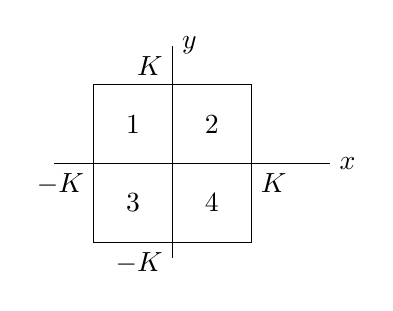
\begin{tikzpicture}
\draw(-1.5,0)--(2,0)node[right]{$x$};
\draw(0,-1.2)--(0,1.5)node[right]{$y$};
\draw(-1,-1) rectangle (1,1);
\draw(0,1)node[above left]{$K$};
\draw(0,-1)node[below left]{$-K$};
\draw(-1,0)node[below left]{$-K$};
\draw(1,0)node[below right]{$K$};
\draw(-0.5,0.5)node{$1$};
\draw(0.5,0.5)node{$2$};
\draw(-0.5,-0.5)node{$3$};
\draw(0.5,-0.5)node{$4$};
\end{tikzpicture}
\caption{مسئلہ \حوالہ{مسئلہ_ترتیب_بلزانو_وائشسٹراس} کا ثبوت}
\label{شکل_مسئلہ_ترتیب_بلزانو_وائشسٹراس}
\end{figure}
\انتہا{ثبوت}
%=======================

ہم اب اس حصے کی مرکزی مسئلہ کو پیش کرنے کے قابل ہیں۔

%==============================
\ابتدا{مسئلہ}\شناخت{مسئلہ_ترتیب_کوشی_اصول_مرکوزیت_برائے_ترتیب}\quad \موٹا{(کوشی اصول مرکوزیت برائے ترتیب)}\فرہنگ{کوشی اصول مرکوزیت!برائے ترتیب}\فرہنگ{Cauchy's conversion principle!sequence}\\
ترتیب \عددی{z_1,z_2,z_3,\cdots} صرف اور صرف اس صورت مرکوز ہو گی جب ہر مثبت عدد \عددی{\epsilon>0} کے لئے ہم ایسا عدد \عددی{N} (جو \عددی{\epsilon} پر منحصر ہو سکتا ہے) تلاش کر سکیں کہ \عددی{m>N} اور \عددی{n>N} کے لئے
\begin{align}\label{مساوات_ترتیب_کوشی_اصول_مرکوزیت_برائے_ترتیب}
\abs{z_m-z_n}<\epsilon\quad \quad \quad m>N,\, n>N
\end{align}
ہو؛ (یعنی \عددی{m>N,\,n>N} کی صورت میں دو اجزاء \عددی{z_m,\,z_n} کا ایک دوسرے سے فاصلہ \عددی{\epsilon} سے کم ہو)۔
\انتہا{مسئلہ}
%==========================
\ابتدا{ثبوت}\quad \موٹا{(الف)} \فاصلہء
 فرض کریں کہ ترتیب \عددی{z_, z_2,\cdots} مرکوز ہے اور اس کا حد \عددی{c} ہے۔ تب دیے گئے \عددی{\epsilon>0} کے لئے ہم ایسا \عددی{N} تلاش کر سکتے ہیں  کہ ہر \عددی{n>N} کے لئے  درج ذیل مطمئن ہو گا۔
\begin{align*}
\abs{z_n-c}<\frac{\epsilon}{2}\quad \quad \quad n>N\,\,\text{ہر}
\end{align*}
یوں جب \عددی{m>N,\, n>N} ہوں تب تکونی عدم مساوات کے تحت
\begin{align*}
\abs{z_m-z_n}=\abs{(z_m-c)-(z_n-c)}\le \abs{z_m-c}+\abs{z_n-c}<\frac{\epsilon}{2}+\frac{\epsilon}{2}=\epsilon
\end{align*}
ہو گا یعنی اگر ترتیب مرکوز ہو تب مساوات \حوالہ{مساوات_ترتیب_کوشی_اصول_مرکوزیت_برائے_ترتیب} مطمئن ہو گی۔

\موٹا{(ب)}\فاصلہء اب الٹ چلتے ہوئے دوسرا ثبوت پیش کرتے ہیں۔  ترتیب \عددی{z_1,z_2,\cdots} جو مساوات \حوالہ{مساوات_ترتیب_کوشی_اصول_مرکوزیت_برائے_ترتیب} کو مطمئن کرتا ہو پر غور کرتے ہیں۔ہم پہلے دکھاتے ہیں کہ یہ ترتیب محدود ہے۔ مساوات \حوالہ{مساوات_ترتیب_کوشی_اصول_مرکوزیت_برائے_ترتیب} میں ایک مقررہ \عددی{\epsilon} اور ایک مقررہ \عددی{n=n_0>N} منتخب کریں۔ تب مساوات \حوالہ{مساوات_ترتیب_کوشی_اصول_مرکوزیت_برائے_ترتیب} کہتی ہے کہ ہر \عددی{m>N} کے لئے ہر \عددی{z_m}، رداس \عددی{\epsilon} کے قرص جس کا مرکز \عددی{z_{n_0}} ہو میں پایا جائے گا، اور ترتیب کے اجزاء کی متناہی تعداد قرص کے باہر پائی جائے گی۔اب ظاہر ہے کہ ہم مبدا پر اتنا بڑا دائرہ لے سکتے ہیں کہ  قرص اور \عددی{z_n} کے متناہی تعداد کے وہ اجزاء جو قرص کے باہر ہیں، اس دائرے کے اندر پائے جائیں۔اس سے ظاہر ہے کہ یہ ترتیب محدود ہے، اور مسئلہ بُلزانو اور وائشسٹراس (مسئلہ \حوالہ{مسئلہ_ترتیب_بلزانو_وائشسٹراس}) کے تحت اس ترتیب کا کم از کم ایک تحدیدی نقطہ ہو گا، جس کو ہم \عددی{L} کہتے ہیں۔ 

ہم اب دکھائیں گے کہ یہ ترتیب مرکوز ہے اور اس کا حد \عددی{L} ہے۔تحدیدی نقطہ کی تعریف سے اخذ کیا جا سکتا ہے کہ دیے گئے \عددی{\epsilon>0} کی صورت میں لامتناہی تعداد کی \عددی{n} کے لئے \عددی{\abs{z_n-L}<\tfrac{\epsilon}{2}} ہو گا۔ چونکہ مساوات \حوالہ{مساوات_ترتیب_کوشی_اصول_مرکوزیت_برائے_ترتیب} کسی بھی \عددی{\epsilon>0} کے لئے درست ہے، جب کوئی \عددی{\epsilon>0} دیا گیا ہو ہم ایسا \عددی{N^*} تلاش کر سکتے ہیں کہ کسی بھی \عددی{m>N^*,\,n>N^*} کے کئے 
\عددی{\abs{z_m-z_n}<\tfrac{\epsilon}{2}} ہو۔ایک مقررہ \عددی{n>N^*} یوں منتخب کریں کہ \عددی{\abs{z_n-L}<\tfrac{\epsilon}{2}} ہو اور فرض کریں کہ \عددی{m} ایسا عدد صحیح ہے جو \عددی{N^*} سے بڑا ہو۔تب تکونی عدم مساوات سے
\begin{align*}
\abs{z_m-L}=\abs{(z_m-z_n)+(z_n-L)}\le \abs{z_m-z_n}+\abs{z_n-L}<\frac{\epsilon}{2}+\frac{\epsilon}{2}=\epsilon
\end{align*}
ہو گا، یعنی، تمام \عددی{m>N^*} کے لئے \عددی{\abs{z_m-L}<\epsilon} ہو گا، جو مرکوزیت کی تعریف ہے۔یوں یہ ترتیب مرکوز ہے اور اس کا حد \عددی{L} ہے۔
\انتہا{ثبوت}
%==========================

کسی بھی دیے گئے تسلسل \عددی{w_1+w_2+\cdots} کے جزوی مجموعوں \عددی{s_n} کی ترتیب پر ہم موجودہ مسئلے کا اطلاق کر سکتے ہیں۔ یوں عدم مساوات \حوالہ{مساوات_ترتیب_کوشی_اصول_مرکوزیت_برائے_ترتیب} درج ذیل صورت اختیار کرے گی
\begin{align*}
\abs{s_m-s_n}<\epsilon\quad \quad \quad (m>N,\,n>N)
\end{align*}
یا اگر ہم \عددی{m=n+p} لکھیں تب 
\begin{align*}
\abs{s_{n+p}-s_n}<\epsilon\quad \quad \quad (n>N,\,p=1,2,\cdots)
\end{align*}
صورت اختیار کرے گی۔اب جزوی مجموعہ کی تعریف سے درج ذیل ہو گا۔
\begin{align*}
s_{n+p}-s_n=w_{n+1}+w_{n+2}+\cdots+w_{n+p}
\end{align*}
اس سے درج ذیل بنیادی مسئلہ ثابت ہوتا ہے۔

%================
\ابتدا{مسئلہ}\شناخت{مسئلہ_ترتیب_کوشی_اصول_مرکوزیت_برائے_تسلسل}\quad \موٹا{(کوشی اصول مرکوزیت برائے تسلسل)}\فرہنگ{کوشی اصول مرکوزیت!تسلسل}\فرہنگ{Cauchy's conversion principle!series}\\
تسلسل \عددی{w_1+w_2+\cdots} صرف اور صرف اس صورت مرتکز ہو گا جب ہر دیے گئے \عددی{\epsilon>0} (جو جتنا کم کیوں نہ ہو) کے لئے ہم ایسا \عددی{N} (جو عموماً \عددی{\epsilon} پر منحصر ہو گا) تلاش کر سکیں کہ ہر \عددی{n>N} اور \عددی{p=1,2,\cdots} کے لئے درج ذیل مطمئن ہو۔
\begin{align*}
\abs{w_{n+1}+w_{n+2}+\cdots+w_{n+p}}<\epsilon \quad \quad n>N,\,\, p=1,2,\cdots 
\end{align*}
\انتہا{مسئلہ}
%============================

اس اہم مسئلے کی پہلی استعمال کے طور پر ہم مسئلہ \حوالہ{مسئلہ_ترتیب_حتمی_مرتکز_مرکوز_ہو_گا} کو ثابت کرتے ہیں۔

%================
\ابتدا{مسئلہ}\شناخت{مسئلہ_ترتیب_کوشی_اصول_استعمال_الف}\quad
اگر تسلسل \عددی{w_1+w_2+\cdots} حتمی مرتکز ہو تب یہ تسلسل مرتکز ہو گا۔
\انتہا{مسئلہ}
%====================
\ابتدا{ثبوت}\quad
عمومی عدم مساوات \حوالہ{مساوات_مخلوط_عدم_مساوات_ب} سے درج ذیل ہو گا۔
\begin{align}\label{مساوات_ترتیب_حتمی_مرتکز_اور_مرتکز_الف}
\abs{w_{n+1}+\cdots+w_{n+p}}\le \abs{w_{n+1}}+\abs{w_{n+2}}+\cdots+\abs{w_{n+p}}
\end{align}
چونکہ ہم فرض کر چکے ہیں کہ تسلسل \عددی{\abs{w_1}+\abs{w_2}+\cdots} مرتکز ہے  لہٰذا مسئلہ \حوالہ{مسئلہ_ترتیب_کوشی_اصول_مرکوزیت_برائے_تسلسل} کے تحت  مساوات \حوالہ{مساوات_ترتیب_حتمی_مرتکز_اور_مرتکز_الف} کا دایاں ہاتھ   ہر \عددی{n>N} (جہاں \عددی{N} کافی بڑا ہے) اور \عددی{p=1,2,\cdots} کے لئے کسی بھی دیے گئے \عددی{\epsilon>0} سے چھوٹا ہو گا۔ یوں یہی کچھ مساوات \حوالہ{مساوات_ترتیب_حتمی_مرتکز_اور_مرتکز_الف} کے بائیں ہاتھ کے لئے بھی درست ہو گا لہٰذا، اسی مسئلہ کے تحت، تسلسل \عددی{w_1+w_2+\cdots} مرتکز ہو گا۔
\انتہا{ثبوت}
%=====================

\حصہء{سوالات}
 کیا سوال \حوالہ{سوال_ترتیب_مرکوزیت_حد_اور_تحدیدی_نقطہ_الف} تا سوال \حوالہ{سوال_ترتیب_مرکوزیت_حد_اور_تحدیدی_نقطہ_ب} میں دیے گئے  ترتیب \عددی{z_1,z_2,\cdots,z_n,\cdots} محدود ہیں؟ مرتکز ہیں؟ ان کے تحدیدی نقطے تلاش کریں۔ 

%=====================
\ابتدا{سوال}\شناخت{سوال_ترتیب_مرکوزیت_حد_اور_تحدیدی_نقطہ_الف}\quad
$z_n=(i2)^n$\\
جواب:\quad
غیر محدود، منفرج، کوئی نہیں
\انتہا{سوال}
%=======================
\ابتدا{سوال}\quad
$z_n=1+i^n$\\
جواب:\quad
محدود، منفرج، \عددی{0,2,1+i,1-i}
\انتہا{سوال}
%=======================
\ابتدا{سوال}\quad
$z_n=(-1)^n+\tfrac{i}{n}$\\
جواب:\quad
محدود، منفرج، \عددی{1,-1}
\انتہا{سوال}
%=======================
\ابتدا{سوال}\quad
$z_n=e^{\tfrac{in\pi}{2}}$\\
جواب:\quad
محدود، منفرج، \عددی{1,-1,i,-i}
\انتہا{سوال}
%=======================
\ابتدا{سوال}\quad
$z_n=i^n\cos n\pi$\\
جواب:\quad
محدود، منفرج، \عددی{1,-1,i,-i}
\انتہا{سوال}
%=======================
\ابتدا{سوال}\quad
$z_n=i^n\cosh n\pi$\\
جواب:\quad
غیر محدود، منفرج، کوئی نہیں
\انتہا{سوال}
%=======================
\ابتدا{سوال}\quad
$z_n=(1-i)^n$\\
جواب:\quad
غیر محدود، منفرج، کوئی نہیں
\انتہا{سوال}
%=======================
\ابتدا{سوال}\quad
$z_n=(1+i)^{2n}$\\
جواب:\quad
غیر محدود، منفرج، کوئی نہیں
\انتہا{سوال}
%=======================
\ابتدا{سوال}\quad
$z_n=\tfrac{(3+i4)^n}{n!}$\\
جواب:\quad
محدود، مرتکز، \عددی{0}
\انتہا{سوال}
%=======================
\ابتدا{سوال}\quad
$z_n=i\pi+\sin n\pi$\\
جواب:\quad
محدود، مرتکز، \عددی{i\pi}
\انتہا{سوال}
%======================
\ابتدا{سوال}\quad
$z_n=\tfrac{\cos n\pi}{\sqrt{n}}$\\
جواب:\quad
محدود، مرتکز، \عددی{0}
\انتہا{سوال}
%======================
\ابتدا{سوال}\quad
$z_n=i^n n^2$\\
جواب:\quad
غیر محدود، منفرج، کوئی نہیں
\انتہا{سوال}
%======================
\ابتدا{سوال}\quad
$z_1=1,z_2=2,z_3=3,z_n=z_{n-3}-z_{n-2}+z_{n-1}\quad (n=4,5,\cdots)$\\
جواب:\quad
محدود، منفرج، \عددی{1,2,3}
\انتہا{سوال}
%=========================
\ابتدا{سوال}\quad
$z_1=\tfrac{1}{3},z_2=\tfrac{1}{4},z_n=\tfrac{z_{n-2}}{z_{n-1}}\quad (n=3,4,\cdots)$\\
جواب:\quad
غیر محدود، منفرج، \عددی{0}
\انتہا{سوال}
%=========================
\ابتدا{سوال}\شناخت{سوال_ترتیب_مرکوزیت_حد_اور_تحدیدی_نقطہ_ب}\quad
$z_1=1,z_2=i,z_n=z_{n-2}z_{n-1}\quad (n=3,2,\cdots)$\\
جواب:\quad
محدود، منفرج، \عددی{1,-1,i,-i}
\انتہا{سوال}
%=========================

\حصہ{یک سر حقیقی ترتیب۔لیبنٹز آزمائش برائے حقیقی تسلسل}\شناخت{حصہ_ترتیب_لیبنٹز_آزمائش_برائے_حقیقی_تسلسل}
اس حصے میں حقیقی ترتیب اور حقیقی تسلسل کے دو مسئلے پیش کیے گئے ہیں جن کے مخلوط ترتیب اور مخلوط تسلسل کے مماثل مسئلے نہیں پائے جاتے ہیں۔دونوں مسئلے عملاً بہت اہم ہیں۔

ایسی حقیقی ترتیب \عددی{x_1,x_2,\cdots,x_n,\cdots}  جس میں
\begin{align*}
x_1\le x_2\le x_3\le\cdots
\end{align*} 
ہو \اصطلاح{یک سر بڑھتی}\فرہنگ{یک سر!بڑھتی}\حاشیہب{monotone increasing}\فرہنگ{monotone!increasing} کہلاتی ہے۔اسی طرح  اگر
\begin{align*}
x_1\ge x_2\ge x_3\ge\cdots
\end{align*} 
ہو تب یہ \اصطلاح{یک سر گھٹتی}\فرہنگ{یک سر!گھٹتی}\حاشیہب{monotone decreasing}\فرہنگ{monotone!decreasing} کہلائے گی۔یک سر بڑھتی یا یک سر گھٹتی ترتیب
 کو  \اصطلاح{یک سر ترتیب}\فرہنگ{یک سر!ترتیب}\فرہنگ{ترتیب!یک سر}\حاشیہب{monotone sequence}\فرہنگ{monotone!sequence} کہتے ہیں۔

مثلاً منفرج ترتیب \عددی{1,2,3,\cdots} یک سر اور غیر محدود ہے۔مرتکز ترتیب \عددی{\tfrac{1}{2},\tfrac{2}{3},\tfrac{3}{4},\cdots} یک سر اور محدود ہے، اور ہم ثابت کریں گے کہ یہ دو خواص مرکوزیت کے لئے کافی ہیں:

%=============================
\ابتدا{مسئلہ}\شناخت{مسئلہ_ترتیب_حقیقی_ترتیب_مرکوزیت}\quad \موٹا{(حقیقی ترتیب کی مرکوزیت)}\فرہنگ{مرکوزیت!حقیقی ترتیب}\فرہنگ{conversion!real sequences}\\
محدود اور یک سر حقیقی ترتیب مرکوز ہو گی۔
\انتہا{مسئلہ}
%===========================
\ابتدا{ثبوت}\quad
فرض کریں کہ \عددی{x_1,x_2,\cdots} محدود یک سر ترتیب ہے۔تب اس کے اجزاء کسی عدد \عددی{B} سے چھوٹے ہوں گے اور، چونکہ، تمام \عددی{n} کے لئے \عددی{x_1\le x_n} ہے لہٰذا تمام اجزاء  وقفہ \عددی{x_1\le x_n\le B} میں پائے جائیں گے جس کو ہم \عددی{I_0} سے ظاہر کرتے ہیں۔ہم  وقفہ \عددی{I_0} کو دو برابر لمبائی کے ٹکڑوں میں تقسیم کرتے ہیں۔اگر \عددی{I_0} کے دائیں نصف (بشمول اس کے دونوں سر) میں ترتیب کے اجزاء پائے جاتے ہوں تب اس ٹکڑے کو ہم \عددی{I_1} سے ظاہر کرتے ہیں۔اگر اس میں ترتیب کے اجزاء نہ پائے جاتے ہوں تب ہم \عددی{I_0} کے بائیں نصف (بشمول اس کے دونوں سر) کو ہم \عددی{ِI_1} سے ظاہر کرتے ہیں۔ یہ پہلا قدم ہے
 (شکل \حوالہ{شکل_مسئلہ_ترتیب_حقیقی_ترتیب_مرکوزیت})۔

دوسرے قدم پر ہم \عددی{ِI_1} کو برابر لمبائی کے دو ٹکڑوں میں تقسیم کرتے ہوئے اسے اصول کے تحت \عددی{I_2} منتخب کرتے ہیں۔

\begin{figure}
\centering
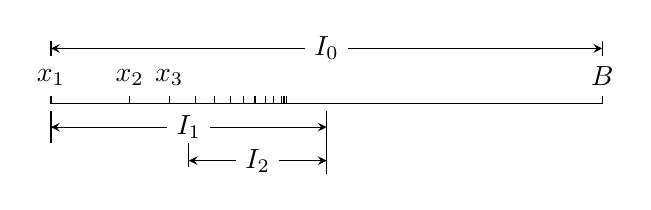
\begin{tikzpicture}
\draw(0,0)--(7,0);
\foreach \x in {0,1,1.5,1.833,2.08,2.283,2.45,2.59,2.72,2.83,2.93,2.95,2.97,2.99,7}{\draw(\x,0)--++(0,0.1);}
\draw(0,0.1)node[above]{$x_1$};
\draw(1,0.1)node[above]{$x_2$};
\draw(1.5,0.1)node[above]{$x_3$};
\draw(7,0.1)node[above]{$B$};
\draw(0,0.6)--++(0,0.2)coordinate[pos=0.5](kA);
\draw(7,0.6)--++(0,0.2);
\draw[stealth-stealth] (kA)--++(7,0)node[pos=0.5,fill=white]{$I_0$};
\draw(0,-0.1)--++(0,-0.4);
\draw(3.5,-0.1)--++(0,-0.8);
\draw[stealth-stealth](0,-0.3)--++(3.5,0)node[pos=0.5,fill=white]{$I_1$};
\draw(3.5/2,-0.5)--(3.5/2,-0.8)coordinate[pos=0.75](kB);
\draw[stealth-stealth] (kB)--++(3.5/2,0)node[pos=0.5,fill=white]{$I_2$};
\end{tikzpicture}
\caption{شکل برائے ثبوت مسئلہ \حوالہ{مسئلہ_ترتیب_حقیقی_ترتیب_مرکوزیت}}
\label{شکل_مسئلہ_ترتیب_حقیقی_ترتیب_مرکوزیت}
\end{figure}

اسی طرح چلتے ہوئے  ہمیں بتدریج چھوٹے وقفے \عددی{I_0, I_1, I_2,\cdots} ملتے ہیں جن کے خواص کچھ یوں ہیں: \عددی{n>m} کی صورت میں  \عددی{I_m} میں تمام \عددی{I_n} شامل ہیں۔ ترتیب کا کوئی جزو \عددی{I_m} کے دائیں جانب نہیں پایا جاتا ہے اور چونکہ ترتیب یک سر بڑھتی ہے، کسی عدد \عددی{N} (جو عموماً \عددی{m} پر منحصر ہو گا) سے زیادہ تمام \عددی{n} کے لئے \عددی{x_n} وقفہ \عددی{I_m} میں پائے جاتے ہیں۔جیسے جیسے \عددی{m} لامتناہی تک پہنچتا ہو ویسے ویسے \عددی{I_m} کی لمبائی صفر کو پہنچتی ہے۔یوں واحد ایک عدد ایسا ہو گا جو ان تمام وقفوں میں پایا جائے گا\حاشیہد{یہ فقرہ صریحاً درست معلوم ہوتا ہے، لیکن حقیقت میں ایسا نہیں ہے۔یہ درحقیقت حقیقی اعدادی نظام کا درج ذیل صورت میں ایک مسلمہ ہے۔فرض کریں کہ \عددی{J_1,J_2,\cdots} ایسے بند وقفے ہیں کہ \عددی{n>m} کے لئے تمام \عددی{J_n} وقفہ \عددی{J_m}  شامل ہوں اور \عددی{m} کی قیمت لامتناہی تک پہنچنے سے \عددی{J_m} کی لمبائی صفر تک پہنچتی ہو۔تب ایسا واحد ایک حقیقی عدد ہو گا جو ان تمام وقفوں میں پایا جائے گا۔اس کو مسلمہ کنتور اور دے دے کند کہتے ہیں جو دو جرمن ریاضی دان گیورگ کنتور [1845-1918] جنہوں نے  نظریہ سلسلہ ایجاد کیا اور  رشارت دے دے کند [1831-1916] کے نام  ہے۔(ایسا وقفہ جس کے سر بھی وقفے میں شامل ہوں بند وقفہ کہلاتا ہے جبکہ وہ وقفہ جس کے سر وقفہ کا حصہ نہ ہوں، کھلا وقفہ کہلاتا ہے۔)}\شناخت{مسلمہ_ترتیب_کنتور_دے_دے_کند}۔اس عدد کو ہم \عددی{L} کہتے ہیں۔ہم اب با آسانی ثابت کر سکتے ہیں کہ یہ ترتیب مرتکز ہے اور اس کا حد \عددی{L} ہے۔

ہم ایسا \عددی{m} منتخب کرتے ہیں کہ \عددی{I_m} کی لمبائی کسی بھی دیے عدد \عددی{\epsilon>0} سے کم ہو۔یوں \عددی{L} اور تمام \عددی{x_n}، جہاں \عددی{n>N(m)} ہے، \عددی{I_m} میں پائے جائیں گے، اور، یوں ان تمام \عددی{n} کے لئے \عددی{\abs{x_n-L}<\epsilon} ہو گا۔یوں بڑھتی ترتیب کے لئے ثبوت مکمل ہوتا ہے۔گھٹتی ترتیب کے لئے ثبوت بالکل ایسا ہی ہے پس وقفوں کی انتخاب کے دوران دائیں کی جگہ بائیں اور بائیں کی جگہ دائیں کا لفظ استعمال کریں۔
\انتہا{ثبوت}
%======================

ہم ایسے حقیقی تسلسل کے ایک اہم مسئلہ کو اب ثابت کرتے ہیں جس کے اجزاء کی علامت متواتر بدلتی ہے اور جس کے اجزاء کی حتمی قیمت بتدریج گھٹتی ہے۔یہ مسئلہ مرکوزیت کے لئے درکار کافی شرائط  اور تسلسل کے باقی کا تخمینہ پیش کرتا ہے

%==========================
\ابتدا{مسئلہ}\شناخت{مسئلہ_ترتیب_آزمائش_لیبنٹز}\quad \موٹا{لیبنٹز آزمائش برائے حقیقی تسلسل}\فرہنگ{آزمائش!لبنیٹز}\فرہنگ{لبنیٹز آزمائش}\فرہنگ{test!Leibniz}\\
فرض کریں کہ حقیقی \عددی{u_1,u_2,\cdots} درج ذیل کو مطمئن کرتے ہیں۔
\begin{align}\label{مسئلہ_ترتیب_آزمائش_لیبنٹز_الف}
\text{(الف)}\quad u_1\ge u_2\ge u_3\ge \cdots,\quad \quad \text{(ب)}\quad \lim_{m\to\infty} u_m=0
\end{align}
تب تسلسل
\begin{align*}
u_1-u_2+u_3-u_4+-\cdots
\end{align*}
مرتکز ہو گی اور \عددی{n} اجزاء کے بعد تسلسل کا باقی کا تخمینہ درج ذیل ہو گا۔
\begin{align}\label{مسئلہ_ترتیب_آزمائش_لیبنٹز_ب}
\abs{R_n}\le u_{n+1}
\end{align}
\انتہا{مسئلہ}
%==================================
\ابتدا{ثبوت}\quad
فرض کریں کہ \عددی{s_n} تسلسل کا \عددی{n} واں جزوی مجموعہ ہے۔تب  مساوات \حوالہ{مسئلہ_ترتیب_آزمائش_لیبنٹز_الف}-الف کے تحت 
\begin{gather*}
\begin{aligned}
s_1&=u_1,\\
s_3&=s_2+u_3\ge s_2,
\end{aligned}\quad
\begin{aligned}
 s_2&=u_1-u_2\le s_1,\\
 s_3&=s_1-(u_2-u_3)\le s_1,
\end{aligned}
\end{gather*}
ہوں گے لہٰذا \عددی{s_2\le s_3\le s_1} ہو گا۔اسی طرح چلتے ہوئے ہم درج ذیل نتیجہ اخذ کرتے ہیں (شکل \حوالہ{شکل_مسئلہ_ترتیب_آزمائش_لیبنٹز})
\begin{align}\label{مسئلہ_ترتیب_آزمائش_لیبنٹز_پ}
s_1\ge s_3\ge s_5\ge \cdots\ge s_6\ge s_4\ge s_2
\end{align}
جس کے تحت طاق جزوی مجموعے محدود یک سر ترتیب بناتے ہیں اور ایسا ہی جفت جزوی مجموعے کرتے ہیں۔یوں مسئلہ \حوالہ{مسئلہ_ترتیب_حقیقی_ترتیب_مرکوزیت} کے تحت دونوں ترتیب مرتکز ہوں گے مثلاً:
\begin{align*}
\lim_{n\to\infty} s_{2n+1}=s,\quad \lim_{n\to\infty} s_{2n}=s^*
\end{align*} 
اب چونکہ \عددی{s_{2n+1}-s_{2n}=u_{2n+1}} ہے لہٰذا ہم دیکھ سکتے ہیں کہ مساوات \حوالہ{مسئلہ_ترتیب_آزمائش_لیبنٹز_الف}-ب سے مراد 
\begin{align*}
s-s^*=\lim_{n\to\infty}s_{2n+1}-\lim_{n\to\infty}s_{2n}=\lim_{n\to\infty}(s_{2n+1}-s_{2n})=\lim_{n\to\infty} u_{2n+1}=0
\end{align*}
ہے۔اس طرح  \عددی{s=s^*} ہو گا لہٰذا  ترتیب مرتکز ہے اور اس کا حد \عددی{s} ہو گا۔

ہم اب مساوات \حوالہ{مسئلہ_ترتیب_آزمائش_لیبنٹز_ب} ثابت کرتے ہیں جو تسلسل کے باقی کا تخمینہ پیش کرتا ہے۔چونکہ \عددی{s_n\to s} ہے  لہٰذا مساوات \حوالہ{مسئلہ_ترتیب_آزمائش_لیبنٹز_پ} سے درج ذیل لکھا جا سکتا ہے۔
\begin{align*}
s_{2n+1}\ge s\ge s_{2n},\quad s_{2n-1}\ge s\ge s_{2n} 
\end{align*}
ان سے \عددی{s_{2n}} اور \عددی{s_{2n-1}} تفریق کرتے ہوئے درج ذیل حاصل ہو گا۔
\begin{align*}
s_{2n+1}-s_{2n}\ge s-s_{2n}\ge 0,\quad 0\ge s-s_{2n-1}\ge s_{2n}-s_{2n-1}
\end{align*}
ان میں بایاں عدم مساوات \عددی{u_{2n+1}} کے برابر ہے جبکہ دایاں عدم مساوات \عددی{-u_{2n}} کے برابر ہے  اور عدم مساوات کی علامتوں کے درمیان باقیات \عددی{R_{2n}} اور \عددی{R_{2n-1}} پائے جاتے ہیں۔یوں ان عدم مساوات کو
\begin{align*}
u_{2n+1}\ge R_{2n}\ge 0,\quad 0\ge R_{2n-1}\ge -u_{2n}
\end{align*}  
لکھا جا سکتا ہے اور ہم دیکھتے ہیں کہ ان سے مراد مساوات \حوالہ{مسئلہ_ترتیب_آزمائش_لیبنٹز_ب} ہے۔یوں ثبوت مکمل ہوتا ہے۔
\begin{figure}
\centering
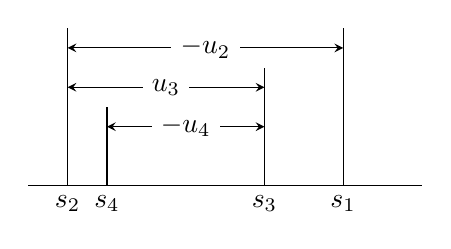
\begin{tikzpicture}
\draw(0,0)--(5,0);
%
\draw(0.5,0)node[below]{$s_2$}--++(0,2);
\draw(1,0)node[below]{$s_4$}--++(0,1);
\draw(3,0)node[below]{$s_3$}--++(0,1.5);
\draw(4,0)node[below]{$s_1$}--++(0,2);
%
\draw[stealth-stealth](1,0.75)--(3,0.75)node[pos=0.5,fill=white]{$-u_4$};
\draw[stealth-stealth](0.5,1.25)--(3,1.25)node[pos=0.5,fill=white]{$u_3$};
\draw[stealth-stealth](0.5,1.75)--(4,1.75)node[pos=0.5,fill=white]{$-u_2$};
\end{tikzpicture}
\caption{ثبوت مسئلہ \حوالہ{مسئلہ_ترتیب_آزمائش_لیبنٹز} (لیبنٹز آزمائش)}
\label{شکل_مسئلہ_ترتیب_آزمائش_لیبنٹز}
\end{figure}
\انتہا{ثبوت}
%============================

\حصہء{سوالات}
کیا سوال \حوالہ{سوال_ترتیب_محدود_یک_سر_تحدیدی_نقطہ_الف} تا سوال \حوالہ{سوال_ترتیب_محدود_یک_سر_تحدیدی_نقطہ_ب} میں دیے ترتیب محدود ہیں؟ مرتکز ہیں؟ یک سر ہیں؟ ان کے تحدیدی نقطے تلاش کریں۔ 

%===============
\ابتدا{سوال}\شناخت{سوال_ترتیب_محدود_یک_سر_تحدیدی_نقطہ_الف}\quad
$1,\tfrac{1}{3},\tfrac{1}{9},\tfrac{1}{27},\cdots$\\
جواب:\quad
محدود، مرتکز، یک سر، \عددی{0}
\انتہا{سوال}
%=======================
\ابتدا{سوال}\quad
$2,-\tfrac{1}{2},3,-\tfrac{1}{3},4,-\tfrac{1}{4},\cdots$\\
جواب:\quad
غیر محدود، منفرج، یک سر، \عددی{0}
\انتہا{سوال}
%=======================
\ابتدا{سوال}\quad
$2,2^2,2^3,2^4,\cdots$\\
جواب:\quad
غیر محدود، منفرج، یک سر، کوئی نہیں
\انتہا{سوال}
%=======================
\ابتدا{سوال}\quad
$1,\sqrt{2},\sqrt[\leftroot{-2}3]3,\sqrt[\leftroot{-2}4]4,\cdots$\\
جواب:\quad
محدود، مرتکز، غیر یک سر، \عددی{1}
\انتہا{سوال}
%=======================
\ابتدا{سوال}\quad
$\tfrac{7}{6},\tfrac{11}{6},\tfrac{8}{7},\tfrac{13}{7},\tfrac{15}{8},\cdots$\\
جواب:\quad
محدود، منفرج، غیر یک سر، \عددی{1,2}
\انتہا{سوال}
%=======================
\ابتدا{سوال}\quad
$\ln 1, \ln 2,\ln 3,\cdots$\\
جواب:\quad
غیر محدود، منفرج، یک سر، کوئی نہیں
\انتہا{سوال}
%=======================
\ابتدا{سوال}\quad
$\tfrac{4}{1!},\tfrac{4^2}{2!},\tfrac{4^3}{3!},\cdots$\\
جواب:\quad
محدود، مرتکز، غیر یک سر، \عددی{0}
\انتہا{سوال}
%=======================
\ابتدا{سوال}\quad
$a,a^2,a^3,\cdots$\\
جواب:\quad
اگر \عددی{a>1} ہو تب غیر محدود، منفرج، یک سر؛ اگر \عددی{0<a<1} ہو تب محدود، مرتکز، یک سر، \عددی{0}؛ اگر \عددی{a=1} ہو تب محدود، منفرج، یک سر، \عددی{1}؛ اگر \عددی{a=-1} ہو تب محدود، منفرج، غیر یک سر، \عددی{1,-1}؛ اگر \عددی{a<-1} ہو تب غیر محدود، منفرج، غیر یک سر  
\انتہا{سوال}
%=======================
\ابتدا{سوال}\quad
$c, 2c^2,3c^3,\cdots \quad (\abs{c}<1)$\\
جواب:\quad
محدود، مرتکز، تحدیدی نقطہ \عددی{0} اور \عددی{0\le c\le \tfrac{1}{2}} کی صورت میں یک سر
\انتہا{سوال}
%=======================
\ابتدا{سوال}\شناخت{سوال_ترتیب_محدود_یک_سر_تحدیدی_نقطہ_ب}\quad
$c,2^2c^2, 3^2c^3,4^2c^4,\cdots\quad (\abs{c}<1)$\\
\انتہا{سوال}
%=======================
کیا سوال \حوالہ{سوال_ترتیب_تسلسل_مرتکز_یا_منفرج_الف} تا سوال \حوالہ{سوال_ترتیب_تسلسل_مرتکز_یا_منفرج_ب} میں دی گئی تسلسل مرتکز یا منفرج ہے؟

%=============
\ابتدا{سوال}\شناخت{سوال_ترتیب_تسلسل_مرتکز_یا_منفرج_الف}\quad
$1-\tfrac{1}{3}+\tfrac{1}{9}-\tfrac{1}{27}+-\cdots$\\
جواب:\quad
مرتکز
\انتہا{سوال}
%=======================
\ابتدا{سوال}\quad
$1-\tfrac{1}{\sqrt{2}}+\tfrac{1}{\sqrt{3}}-\tfrac{1}{\sqrt{4}}+-\cdots$\\
جواب:\quad
مرتکز
\انتہا{سوال}
%=======================
\ابتدا{سوال}\quad
$\tfrac{3}{2}-\tfrac{4}{3}+\tfrac{5}{4}-\tfrac{6}{5}+-\cdots$\\
جواب:\quad
مسئلہ \حوالہ{مسئلہ_ترتیب_مرکوزیت_شرط} کے تحت منفرج  ہے
\انتہا{سوال}
%=======================
\ابتدا{سوال}\شناخت{سوال_ترتیب_تسلسل_مرتکز_یا_منفرج_ب}\quad
$\tfrac{1}{\ln 2}+\tfrac{1}{\ln 3}+\tfrac{1}{\ln 4}+\cdots$
\انتہا{سوال}
%=========================
دکھائیں کہ سوال \حوالہ{سوال_ترتیب_ارکان_درکار_الف} تا سوال \حوالہ{سوال_ترتیب_ارکان_درکار_ب} میں دیے گئے تسلسل مرتکز ہیں۔تسلسل کے مجموعہ \عددی{s} میں خلل \عددی{\epsilon} کو \عددی{0.01} سے کم رکھنے کی خاطر تسلسل کے کتنے اجزاء درکار ہوں گے؟

%==================
\ابتدا{سوال}\شناخت{سوال_ترتیب_ارکان_درکار_الف}\quad
$s=\tfrac{1}{2}-\tfrac{1}{4}+\tfrac{1}{8}-+\cdots$\\
جواب:\quad 
$6$
\انتہا{سوال}
%=====================
\ابتدا{سوال}\quad
$s=1-\tfrac{1}{3}+\tfrac{1}{6}-\tfrac{1}{12}+\tfrac{1}{24}-+\cdots$\\
$6$
\انتہا{سوال}
%=====================
\ابتدا{سوال}\quad
$s=1-\tfrac{1}{3}+\tfrac{1}{9}-\tfrac{1}{27}+-\cdots$\\
جواب:\quad
$5$
\انتہا{سوال}
%========================
\ابتدا{سوال}\quad
$s=1-1+\tfrac{1}{2!}-\tfrac{1}{3!}+\tfrac{1}{4!}-+\cdots$
\انتہا{سوال}
%=======================
\ابتدا{سوال}\quad
$s=1-\tfrac{1}{3!}+\tfrac{1}{5!}-\tfrac{1}{7!}+-\cdots$\\
جواب:\quad
$2$
\انتہا{سوال}
%==========================
\ابتدا{سوال}\شناخت{سوال_ترتیب_ارکان_درکار_ب}\quad
$s=1-\tfrac{1}{2!}+\tfrac{1}{4!}-\tfrac{1}{6!}+-\cdots$
\انتہا{سوال}
%==========================

\حصہ{تسلسل کی مرکوزیت اور انفراج کی آزمائشیں}\شناخت{حصہ_ترتیب_تسلسل_آزمائش}
کسی بھی تسلسل کو حساب یا دیگر مقاصد کے لئے استعمال کرنے سے پہلے اس کی مرکوزیت جاننا ضروری ہے۔انجینئری حساب کے مسائل میں اس کا جواب عموماً مرکوزیت اور انفراج کے دیگر آزمائشوں\حاشیہب{tests} میں سے کسی ایک کے اطلاق سے حاصل کرنا ممکن ہو گا۔یوں مرکوزیت اور انفراج کی آزمائشیں عملاً نہایت اہم ہیں۔

حقیقی تسلسل کی انفراج کی آزمائش کے سادہ اصول مسئلہ \حوالہ{مسئلہ_ترتیب_آزمائش_مرکوزیت_حقیقی} اور لیبنٹز آزمائش پر ہم پہلے غور کر چکے ہیں۔ درج ذیل مسئلہ مرکوزیت کی دیگر آزمائشوں کا جواز ہے۔

%==================
\ابتدا{مسئلہ}\شناخت{مسئلہ_ترتیب_جانچ_مقابلہ}\quad \موٹا{تقابلی آزمائش}\فرہنگ{آزمائش!تقابلی}\فرہنگ{test!comparison}\\
اگر تسلسل \عددی{w_1+w_2+\cdots} دیا گیا ہو اور ہم غیر منفی اجزاء والا ایسا تسلسل \عددی{b_1+b_2+\cdots} تلاش کر سکیں کہ
\begin{align}\label{مساوات_ترتیب_جانچ_مقابلہ_الف}
\abs{w_n}\le b_n\quad n=1,2,\cdots
\end{align}
ہو تب دیا گیا تسلسل حتمی مرتکز ہو گا۔
\انتہا{مسئلہ}
%======================
\ابتدا{ثبوت}\quad
چونکہ تسلسل \عددی{b_1+b_2+\cdots} مرتکز ہے  لہٰذا مسئلہ \حوالہ{مسئلہ_ترتیب_کوشی_اصول_مرکوزیت_برائے_تسلسل} کے تحت کسی بھی دیے گئے \عددی{\epsilon>0} کے لئے ہم ایسا \عددی{N} تلاش کر سکتے ہیں کہ ہر \عددی{n>N} اور \عددی{p=1,2,\cdots} کے لئے درج ذیل ہو گا۔
\begin{align*}
b_{n+1}+\cdots+b_{n+p}<\epsilon \quad \quad n>N,\quad p=1,2,\cdots
\end{align*}
اس کو مساوات \حوالہ{مساوات_ترتیب_جانچ_مقابلہ_الف} کے ساتھ ملا کر ان \عددی{n} اور \عددی{p} کے لئے درج ذیل اخذ کیا جا سکتا ہے۔
\begin{align*}
\abs{w_{n+1}}+\cdots+\abs{w_{n+p}}\le b_{n+1}+\cdots+b_{n+p}<\epsilon
\end{align*}
یوں مسئلہ \حوالہ{مسئلہ_ترتیب_کوشی_اصول_مرکوزیت_برائے_تسلسل} کے تحت تسلسل \عددی{\abs{w_1}+\abs{w_2}+\cdots} مرتکز ہو گا اور دیا گیا تسلسل حتمی مرتکز ہو گا۔
\انتہا{ثبوت}
%======================

مسئلہ \حوالہ{مسئلہ_ترتیب_جانچ_مقابلہ} سے دو اہم آزمائشیں  اخذ کرنے کی خاطر درج ذیل ثابت کرتے ہیں۔

%====================
\ابتدا{مسئلہ}\شناخت{مسئلہ_ترتیب_ہندسی_تسلسل}\quad \موٹا{ہندسی تسلسل}\فرہنگ{ہندسی!تسلسل}\فرہنگ{geometric!series}\\
\عددی{\abs{q}<1} کی صورت میں ہندسی تسلسل
\begin{align*}
\sum_{m=0}^{\infty} q^m=1+q+q^2+\cdots
\end{align*}
مرتکز ہو گا اور اس کا مجموعہ \عددی{\tfrac{1}{1-q}} ہو گا جبکہ \عددی{\abs{q}\ge 1} کی صورت میں ہندسی تسلسل منفرج ہو گا۔ 
\انتہا{مسئلہ}
%=========================
\ابتدا{ثبوت}\quad
جب \عددی{\abs{q}\ge 1} ہو تب \عددی{\abs{q^n}\ge 1} ہو گا لہٰذا مسئلہ \حوالہ{مسئلہ_ترتیب_مرکوزیت_شرط} کے تحت تسلسل منفرج ہو گا۔اب \عددی{\abs{q}<1}  کی صورت میں \عددی{n} واں جزوی مجموعہ
\begin{align*}
s_n=1+q+\cdots+q^n
\end{align*}
ہو گا جس کو \عددی{q} سے ضرب دینے سے
\begin{align*}
qs_n=q+q^2+\cdots+q^{n+1}
\end{align*}
ملتا ہے۔ان کی تفریق سے  باقی تمام اجزاء  آپس میں کٹ جاتے ہیں اور
\begin{align*}
s_n-qs_n=(1-q)s_n=1-q^{n+1}
\end{align*}
حاصل ہوتا ہے۔چونکہ \عددی{q\ne 1} ہے لہٰذا \عددی{1-q\ne 0} ہو گا اور یوں ہم \عددی{s_n} کے لئے حل کرتے ہوئے درج ذیل حاصل کرتے ہیں۔
\begin{align}
s_n=\frac{1-q^{n+1}}{1-q}=\frac{1}{1-q}-\frac{q^{n+1}}{1-q}
\end{align}
چونکہ \عددی{\abs{q}<1} ہے لہٰذا \عددی{n\to\infty} کی صورت میں  آخری جزو صفر تک پہنچتا ہے۔یوں تسلسل مرتکز ہے اور اس کی قیمت \عددی{\tfrac{1}{1-q}} ہے۔ 
\انتہا{ثبوت}
%============================

مسئلہ \حوالہ{مسئلہ_ترتیب_جانچ_مقابلہ} اور مسئلہ \حوالہ{مسئلہ_ترتیب_ہندسی_تسلسل} سے دو اہم آزمائشیں، تناسبی آزمائش اور جذری آزمائش حاصل کرتے ہیں۔

%======================
\ابتدا{مسئلہ}\شناخت{مسئلہ_ترتیب_تناسبی_آزمائش}\quad \موٹا{تناسبی آزمائش}\فرہنگ{آزمائش!تناسبی}\فرہنگ{test!ratio}\\
ہم درج ذیل تسلسل پر غور کرتے ہیں۔
\begin{align*}
w_1+w_2+w_3+\cdots
\end{align*}
فرض کریں کہ \عددی{n=1,2,\cdots} کے لئے \عددی{w_n\ne 0} ہے اور درج ذیل تناسب کی ترتیب مرتکز ہے اور اس  کا حد \عددی{L} ہے۔
\begin{align*}
\abs{\frac{w_{n+1}}{w_n}}\quad \quad \quad n=1,2,\cdots
\end{align*}
تب \عددی{L<1} کی صورت میں تسلسل حتمی مرتکز ہے جبکہ \عددی{L>1} کی صورت میں تسلسل منفرج ہے۔ (یہ آزمائش \عددی{L=1} کی صورت میں نا کام ہے اور اس سے کچھ اخذ نہیں کیا جا سکتا ہے۔)
\انتہا{مسئلہ}
%===========================
\ابتدا{ثبوت}\quad
ہم درج ذیل فرض کر چکے ہیں۔
\begin{align*}
\lim_{n\to\infty} k_n=L \quad \quad \quad k_n=\abs{\frac{w_{n+1}}{w_n}}
\end{align*}
ظاہر ہے کہ \عددی{k_n} اور \عددی{L} حقیقی ہیں۔حد کی تعریف کے تحت، کسی بھی دیے گئے \عددی{\epsilon>0} کے لئے ہم ایسا \عددی{N} تلاش کر سکتے ہیں کہ ہر \عددی{n>N} کے لئے \عددی{k_n} وقفہ \عددی{L-\epsilon} تا \عددی{L+\epsilon} پر پایا جاتا ہو یعنی:
\begin{align}\label{مساوات_ترتیب_نسبت_الف}
\text{(الف)}\quad k_n<L+\epsilon \quad \quad \text{(ب)}\quad k_n>L-\epsilon\quad \quad \quad (n>N)
\end{align}
ہم اب \عددی{L<1} کی صورت پر غور کرتے ہیں۔ہم \عددی{L+\epsilon=q} لکھتے ہیں اور \عددی{\epsilon=\tfrac{1-L}{2}} لیتے ہیں۔یوں \عددی{\epsilon>0} ہو گا اور ہم  مساوات \حوالہ{مساوات_ترتیب_نسبت_الف}-الف کو
\begin{align*}
k_n<q=L+\frac{1-L}{2}=\frac{1+L}{2}
\end{align*}
لکھ سکتے ہیں۔چونکہ \عددی{L<1} ہے لہٰذا \عددی{q<1} ہو گا۔اب ہم درج ذیل لکھ سکتے ہیں۔
\begin{multline}\label{مساوات_ترتیب_نسبت_ب}
\abs{w_{N+1}}+\abs{w_{N+2}}+\abs{w_{N+3}}+\cdots\\
=\abs{w_{N+1}}\big(1+\abs{\frac{w_{N+2}}{w_{N+1}}}+\abs{\frac{w_{N+3}}{w_{N+2}}}\abs{\frac{w_{N+2}}{w_{N+1}}}+\cdots\big)\\
=\abs{w_{N+1}}(1+k_{N+1}+k_{N+2}k_{N+1}+k_{N+3}k_{N+2}k_{N+1}+\cdots)
\end{multline}
چونکہ \عددی{k_n<q<1} ہے لہٰذا اس تسلسل کا ہر جزو درج ذیل ہندسی تسلسل کے مطابقتی جزو سے کم ہے۔
\begin{align*}
\abs{w_{N+1}}(1+q+q^2+q^3+\cdots)
\end{align*}
چونکہ \عددی{q<1} ہے لہٰذا مسئلہ \حوالہ{مسئلہ_ترتیب_ہندسی_تسلسل} کے تحت تسلسل مرتکز ہو گا۔مسئلہ \حوالہ{مسئلہ_ترتیب_جانچ_مقابلہ} کے تحت  مساوات \حوالہ{مساوات_ترتیب_نسبت_ب} میں دیا گیا تسلسل مرتکز ہو گا۔یوں تسلسل \عددی{\abs{w_1}+\abs{w_2}+\cdots} مرتکز ہو گا۔اس سے مراد تسلسل \عددی{w_1+w_2+\cdots} کی حتمی مرکوزیت ہے۔

ہم اب \عددی{L>1} کی صورت پر غور کرتے ہیں۔ہم \عددی{\epsilon=\tfrac{L-1}{2}} منتخب کرتے ہیں۔یوں ظاہر ہے کہ \عددی{\epsilon>0} ہو گا اور  مساوات \حوالہ{مساوات_ترتیب_نسبت_الف}-ب درج ذیل صورت اختیار کرتی ہے
\begin{align}
k_n>L-\epsilon=\frac{1+L}{2}>1\quad \quad \quad (n>N)
\end{align}
یعنی:
\begin{align}
k_n=\abs{\frac{w_{n+1}}{w_n}}>1 \quad \implies \quad \abs{w_{n+1}}>\abs{w_n} \quad \quad \quad (n>N)
\end{align}
یہ آخری عدم مساوات کہتی ہے کہ اجزاء کی حتمی قیمت بتدریج بڑھتی ہے لہٰذا مسئلہ \حوالہ{مسئلہ_ترتیب_مرکوزیت_شرط} کے تحت تسلسل منفرج ہو گا۔(\عددی{L=1} کی صورت میں تسلسل مرتکز یا منفرج ہو سکتا ہے اور  تناسبی آزمائش کارآمد نہیں ہو گی۔)
\انتہا{ثبوت}
%==========================

\عددی{L=1} کی صورت میں مرتکز اور منفرج تسلسل کی مثال پیش کرتے ہیں۔ہم مثال \حوالہ{مثال_ترتیب_ہارمونی_منفرج} میں دیکھ چکے ہیں کہ ہارمونی تسلسل 
\begin{align*}
\sum_{n=1}^{\infty} \frac{1}{n}=1+\frac{1}{2}+\frac{1}{3}+\cdots
\end{align*}
منفرج ہے۔اس کے لئے \عددی{n\to \infty} کی صورت میں
\begin{align*}
\frac{w_{n+1}}{w_n}=\frac{n}{n+1}\equiv L=1 \quad \quad n\to \infty
\end{align*}
حاصل ہوتا ہے۔اس کے برعکس درج ذیل تسلسل
\begin{align}\label{مساوات_ترتیب_تسلسل_مربع_بالعکس}
\sum_{n=1}^{\infty}\frac{1}{n^2}=1+\frac{1}{4}+\frac{1}{9}+\cdots
\end{align}
مرتکز ہے جبکہ اس کے لئے
\begin{align*}
\frac{w_{n+1}}{w_n}=\frac{n^2}{(n+1)^2}\equiv L=1\quad \quad n\to\infty
\end{align*}
حاصل ہوتا ہے۔مساوات \حوالہ{مساوات_ترتیب_تسلسل_مربع_بالعکس} کی مرکوزیت ثابت کرتے ہیں۔اس کا \عددی{n} ویں جزوی مجموعہ
\begin{align*}
s_n=1+\frac{1}{4}+\frac{1}{9}+\cdots+\frac{1}{n^2}
\end{align*}
ہو گا۔ظاہر ہے کہ \عددی{s_n>0} ہو گا  اور (شکل \حوالہ{شکل_مساوات_ترتیب_تسلسل_مربع_بالعکس}) 
\begin{align*}
s_n\le 1+\int_{1}^{n}\frac{\dif x}{x^2}=2-\frac{1}{n}
\end{align*}
ہو گا۔اس مساوات کے تحت جزوی مجموعوں کی ترتیب  محدود ہے۔چونکہ تسلسل کے اجزاء مثبت ہیں، تسلسل یک سر بڑھتا  تسلسل ہے  لہٰذا مسئلہ \حوالہ{مسئلہ_ترتیب_حقیقی_ترتیب_مرکوزیت} کے تحت تسلسل مرتکز ہو گا۔
\begin{figure}
\centering
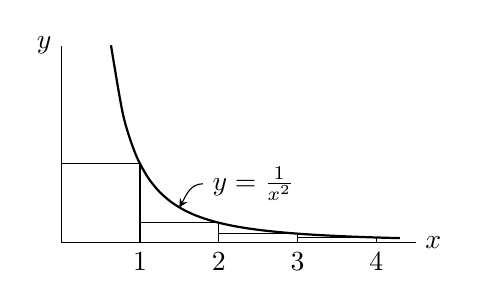
\begin{tikzpicture}
\draw(0,0)--++(4.5,0)node[right]{$x$};
\draw(0,0)--++(0,2.5)node[left]{$y$};
\draw[thick,smooth,domain=0.632:4.3] plot ({\x},{1/\x^2});
\draw(1,0)node[below]{$1$}--++(0,1)--++(-1,0);
\draw(2,0)node[below]{$2$}--++(0,1/4)--++(-1,0);
\draw(3,0)node[below]{$3$}--++(0,1/9)--++(-1,0);
\draw(4,0)node[below]{$4$}--++(0,1/16)--++(-1,0);
\draw[stealth-] (1.5,1/1.5^2) to [out=60,in=180]++(0.3,0.3)node[right]{$y=\frac{1}{x^2}$};
\end{tikzpicture}
\caption{تسلسل \حوالہ{مساوات_ترتیب_تسلسل_مربع_بالعکس} کی مرکوزیت}
\label{شکل_مساوات_ترتیب_تسلسل_مربع_بالعکس}
\end{figure}

درج ذیل تناسبی آزمائش سے  زیادہ عمومی آزمائش  ہے البتہ اس کا استعمال نسبتاً مشکل ثابت ہوتا ہے۔

%=======================
\ابتدا{مسئلہ}\quad \موٹا{جذری آزمائش}\\
درج ذیل تسلسل پر غور کریں۔
\begin{align*}
w_1+w_2+w_3+\cdots
\end{align*}
فرض کریں کہ درج ذیل جذر کی ترتیب
\begin{align*}
\sqrt[\leftroot{-2}n]{\abs{w_n}}\quad \quad \quad n=1,2,\cdots
\end{align*}
مرتکز ہے اور اس کا حد \عددی{L} ہے۔تب \عددی{L<1} کی صورت میں دیا گیا تسلسل حتمی مرتکز ہو گا جبکہ \عددی{L>1} کی صورت میں تسلسل منفرج ہو گا۔ (\عددی{L=1} کی صورت میں آزمائش کارآمد نہیں ہو گی۔)
\انتہا{مسئلہ}
%===========================
\ابتدا{ثبوت}\quad
اگر \عددی{L<1} ہو، تب، تناسبی آزمائش کی طرح، ہم \عددی{q<1} منتخب کرتے ہوئے ایسا مطابقتی \عددی{N} تلاش کرتے ہیں کہ ہر \عددی{n>N} کے لئے درج ذیل مطمئن ہو۔
\begin{align*}
k_n^*\equiv \sqrt[\leftroot{-2}n]{\abs{w_n}}<q<1\quad \quad n>N\, \text{ہر}
\end{align*}
اس سے درج ذیل حاصل ہو گا۔
\begin{align*}
\abs{w_n}<q^n<1\quad \quad \quad (n>N)
\end{align*}
یوں ہندسی تسلسل کے ساتھ موازنہ کرنے سے ہم دیکھتے ہیں کہ تسلسل \عددی{\abs{w_N}+\abs{w_{N+1}}+\cdots} مرتکز ہو گا۔اس طرح تسلسل \عددی{w_1+w_2+\cdots} حتمی مرتکز ہو گا۔

اگر \عددی{L>1} ہو، تب  کافی بڑے \عددی{n} کے لئے 
$\,\sqrt[\leftroot{-2}n]{\abs{w_n}}>1\,$
ہو گا۔یوں ان \عددی{n} کے لئے \عددی{\abs{w_n}>1} ہو گا لہٰذا مسئلہ \حوالہ{مسئلہ_ترتیب_آزمائش_مرکوزیت_حقیقی} کے تحت تسلسل منفرج ہو گا۔

اگر \عددی{L=1} ہو تب آزمائش کارآمد نہیں رہتی ہے۔
\انتہا{ثبوت}
%======================

\عددی{L=1} کی صورت میں آزمائش کی ناقص پن کو دو تسلسلوں کی مدد سے دیکھتے ہیں۔ ہارمونی تسلسل کی صورت میں  \عددی{L=1}  اور
\begin{align*}
\sqrt[\leftroot{-2}n]{\frac{1}{n}}=\frac{1}{n^{\tfrac{1}{n}}}=\frac{1}{e^{(1/n)\ln n}}\to \frac{1}{e^0}=1\quad \quad (n\to \infty)
\end{align*} 
ہو گا، چونکہ \عددی{\tfrac{1}{n}\ln n\to 0} ہے۔ اسی طرح تسلسل \حوالہ{مساوات_ترتیب_تسلسل_مربع_بالعکس} کے لئے \عددی{L=1} اور
\begin{align*}
\sqrt[\leftroot{-2}n]{\frac{1}{n^2}}=\frac{1}{n^{\tfrac{2}{n}}}=\frac{1}{e^{2/n}\ln n}\to \frac{1}{e^0}=1\quad \quad (n\to \infty)
\end{align*}
ہو گا، چونکہ \عددی{\tfrac{2}{n}\ln n\to 0} ہے۔

%============================
\ابتدا{مثال}\quad \موٹا{تناسبی آزمائش اور جذری آزمائش کا عملی استعمال}\\
درج ذیل تسلسل کو آزما کر دیکھیں۔
\begin{align*}
\sum_{n=1}^{\infty} \frac{n^2}{2^n}=\frac{1}{2}+1+\frac{9}{8}+1+\frac{25}{32}+\cdots
\end{align*}
اس تسلسل سے 
\begin{align*}
w_n=\frac{n^2}{2^n}, \quad w_{n+1}=\frac{(n+1)^2}{2^{n+1}},\quad \frac{w_{n+1}}{w_n}=\frac{(n+1)^2}{2n^2}\to \frac{1}{2}\quad (n\to\infty)
\end{align*}
لکھا جا سکتا ہے لہٰذا تناسبی آزمائش کے تحت تسلسل مرتکز ہے۔ہم جذری آزمائش بھی استعمال کر سکتے ہیں:
\begin{align*}
\sqrt[\leftroot{-2}n]{\frac{n^2}{2^n}}=\frac{n^{\tfrac{2}{n}}}{2}=\frac{e^{\tfrac{2}{n}\ln n}}{2}\to \frac{e^0}{2}=\frac{1}{2}\quad (n\to\infty)
\end{align*}
جو وہی نتیجہ ہے۔ 
\انتہا{مثال}
%==============================
\ابتدا{مثال}\quad \موٹا{تناسبی آزمائش کا استعمال}\\
کیا درج ذیل تسلسل مرتکز یا منفرج ہے؟
\begin{align*}
\sum_{n=0}^{\infty}\frac{(3-i4)^n}{n!}=1+(3-i4)+\frac{1}{2!}(3-i4)^2+\cdots
\end{align*}
اس تسلسل سے 
\begin{align*}
\abs{w_n}=\frac{\abs{3-i4}^n}{n!}=\frac{5^n}{n!}, \quad \abs{w_{n+1}}=\frac{5^{n+1}}{(n+1)!},\quad \abs{\frac{w_{n+1}}{w_n}}=\frac{5}{n+1}\to 0 \quad (n\to \infty)
\end{align*}
لکھا جا سکتا ہے۔یوں تناسبی آزمائش کے تحت تسلسل مرتکز ہے۔
\انتہا{مثال}

ہم آخر میں بتلانا چاہتے ہیں کہ تناسبی آزمائش اور جذری آزمائش کو وسعت دیتے ہوئے بالترتیب  ایسے ترتیب جن کے اجزاء \عددی{\abs{\tfrac{w_{n+1}}{w_n}}} اور 
$\,\sqrt[\leftroot{-2}n]{\abs{w_n}}\,$
غیر مرتکز ہوں پر بھی لاگو کیا جا سکتا ہے۔
%===================
\ابتدا{مسئلہ}\شناخت{مسئلہ_ترتیب_تناسبی_آزمائش_ب}\quad \موٹا{تناسبی آزمائش}\\
درج ذیل تسلسل پر غور کریں۔
\begin{align*}
w_!+w_2+w_3+\cdots
\end{align*}
فرض کریں کہ \عددی{n=1,2,\cdots} کے لئے \عددی{w_n\ne 0} ہیں۔ اگر کسی \عددی{N} سے ہر بڑے \عددی{n} کے لئے
\begin{align}\label{مساوات_ترتیب_تناسبی_الف}
\abs{\frac{w_{n+1}}{w_n}}\le q\quad \quad (n>N)
\end{align}
ہو جہاں \عددی{q} اکائی سے کم کوئی مقررہ عدد ہے، تب تسلسل حتمی منفرج ہو گا۔اگر ہر \عددی{n>N} کے لئے 
\begin{align}\label{مساوات_ترتیب_تناسبی_ب}
\abs{\frac{w_{n+1}}{w_n}}\ge 1\quad \quad (n>N)
\end{align}
ہو تب تسلسل منفرج ہو گا۔
\انتہا{مسئلہ}
%=======================
\ابتدا{ثبوت}\quad
مسئلہ \حوالہ{مسئلہ_ترتیب_تناسبی_آزمائش} کے پہلے حصے میں ہر \عددی{n>N} کے لئے ایسے عدد \عددی{q<1} کی موجودگی  جو مساوات \حوالہ{مساوات_ترتیب_تناسبی_الف} کو مطمئن کرتا ہو، مرکوزیت کی وجہ بنی۔یوں موجودہ مسئلے میں بھی مرکوزیت کی یہی وجہ ہے۔مساوات \حوالہ{مساوات_ترتیب_تناسبی_ب} کے تحت \عددی{\abs{w_{n+1}}\ge \abs{w_n}} ہے لہٰذا   مسئلہ \حوالہ{مسئلہ_ترتیب_مرکوزیت_شرط}سے مسئلے کا دوسرا حصہ ثابت ہوتا ہے۔
\انتہا{ثبوت}
%====================

\ابتدا{مثال}\quad \موٹا{مسئلہ \حوالہ{مسئلہ_ترتیب_تناسبی_آزمائش_ب} کا اطلاق۔مسئلہ \حوالہ{مسئلہ_ترتیب_تناسبی_آزمائش} کی نا کامی}\\
تسلسل
\begin{align*}
1+\frac{1}{2}+\frac{1}{8}+\frac{1}{16}+\frac{1}{64}+\frac{1}{128}+\frac{1}{512}+\cdots
\end{align*}
کے طاق اجزاء اور جفت اجزاء دونوں ہندسی تسلسل بناتے ہیں جن کی تناسب \عددی{\tfrac{1}{8}} ہے۔چونکہ قریبی اجزاء کی تناسب
\begin{align*}
\frac{1}{2},\frac{1}{4},\frac{1}{2},\frac{1}{4},\cdots
\end{align*}
ہے لہٰذا مسئلہ \حوالہ{مسئلہ_ترتیب_تناسبی_آزمائش_ب} کے تحت تسلسل مرتکز ہے۔ہم دیکھتے ہیں کہ ان تناسب کی ترتیب مرتکز نہیں ہے لہٰذا  مسئلہ \حوالہ{مسئلہ_ترتیب_تناسبی_آزمائش} یہاں کام نہیں کرے گا۔یوں آپ دیکھ سکتے ہیں کہ مسئلہ \حوالہ{مسئلہ_ترتیب_تناسبی_آزمائش} سے مسئلہ \حوالہ{مسئلہ_ترتیب_تناسبی_آزمائش_ب} زیادہ عمومی ہے۔
\انتہا{مثال}
%=============================
\ابتدا{مسئلہ}\شناخت{مسئلہ_ترتیب_جذری_آزمائش_ب}\quad \موٹا{جذری آزمائش}\\
درج ذیل تسلسل پر غور کریں۔
\begin{align*}
w_!+w_2+w_3+\cdots
\end{align*}
اگر کسی عدد \عددی{N} سے ہر بڑے \عددی{n}  کے لئے
\begin{align}\label{مساوات_ترتیب_جذری_الف}
\sqrt[\leftroot{-2}n]{\abs{w_n}}\le q
\end{align}
ہو جہاں \عددی{q} اکائی سے کم کوئی مقررہ عدد ہے، تب دیا گیا تسلسل حتمی مرتکز ہو گا۔اگر \عددی{n} کی متناہی تعداد اجزاء  کے لئے 
\begin{align}\label{مساوات_ترتیب_جذری_ب}
\sqrt[\leftroot{-2}n]{\abs{w_n}}\ge 1
\end{align}
ہو تب تسلسل منفرج ہو گا۔
\انتہا{مسئلہ}
%==========================
\ابتدا{ثبوت}\quad
اگر مساوات \حوالہ{مساوات_ترتیب_جذری_الف} مطمئن ہو تب کافی بڑے \عددی{n} کے لئے
\begin{align*}
\abs{w_n}\le q^n<1 \quad \quad \quad (n>N)
\end{align*}
ہو گا اور ہندسی تسلسل کے ساتھ موازنہ کرنے سے تسلسل
$\,\abs{w_N}+\abs{w_{N+1}}+\cdots\,$
مرتکز حاصل ہوتا ہے۔یوں تسلسل \عددی{w_1+w_2+\cdots} حتمی مرتکا ہو گا۔اگر مساوات \حوالہ{مساوات_ترتیب_جذری_ب} مطمئن ہو تب \عددی{n} کی متناہی تعداد کے لئے  \عددی{\abs{w_n}\ge 1} ہو گا  لہٰذا مسئلہ \حوالہ{مسئلہ_ترتیب_مرکوزیت_شرط} کے تحت تسلسل منفرج ہو گا۔

\انتہا{ثبوت}
%==========================

درج بالا دونوں مسئلوں میں مرکوزیت کے لئے لازمی ہے کہ بالترتیب \عددی{\abs{\tfrac{w_{n+1}}{w_n}}} اور 
$\,\sqrt[\leftroot{-2}n]{\abs{w_n}}\,$
 کسی مقررہ عدد \عددی{q<1} کے برابر یا اس سے کم ہو۔کسی بھی بڑے \عددی{n} کے لئے مرکوزیت ہرگز   \عددی{\abs{\tfrac{w_{n+1}}{w_n}}<1} یا 
$\,\sqrt[\leftroot{-2}n]{\abs{w_n}}<1\,$
سے اخذ نہیں کی جا سکتی ہے۔

مثال کے طور پر اگرچہ ہارمونی تسلسل \عددی{\sum_{m=1}^{\infty}\tfrac{1}{m}=1+\tfrac{1}{2}+\tfrac{1}{3}+\cdots} کے لئے
\begin{align*}
\sqrt[\leftroot{-2}n]{\frac{1}{n}}<1\quad \text{اور}\quad \frac{w_{n+1}}{w_n}=\frac{\tfrac{1}{n+1}}{\tfrac{1}{n}}=\frac{n}{n+1}<1
\end{align*}
ہیں لیکن تسلسل منفرج ہے۔

یہاں یہ بات سمجھنی ضروری ہے کہ ہارمونی تسلسل کے لئے  ہم \عددی{1} سے کم ایسا کوئی عدد  \عددی{q} منتخب نہیں کر سکتے ہیں کہ  
$\,\sqrt[\leftroot{-2}n]{\frac{1}{n}}<q\,$
یا 
$\,\frac{w_{n+1}}{w_n}=\tfrac{n}{n+1}<q\,$
ہو۔فرض کریں کہ ہم \عددی{q=0.9} منتخب کرتے ہیں۔تب \عددی{n=10} لیتے ہوئے 
$\,\frac{w_{n+1}}{w_n}=\tfrac{10}{10+1}=0.909\,$
حاصل ہوتا ہے جو \عددی{q=0.9} سے کم نہیں ہے۔اسی طرح اگر ہم \عددی{q=0.9999} منتخب کریں تب \عددی{n=10000} لیتے ہوئے 
$\,\frac{w_{n+1}}{w_n}=\tfrac{10000}{10000+1}=0.99990001\,$
حاصل ہوتا ہے جو \عددی{q=0.9999} سے کم نہیں ہے۔آپ دیکھ سکتے ہیں کہ کسی بھی منتخب کردہ \عددی{q\,(<1)}  کے لئے ایسا \عددی{n} پایا جاتا ہے کہ یہ شرط مطمئن نہیں ہوتا ہے۔یوں اگرچہ 
$\,\frac{w_{n+1}}{w_n}<1\,$
ہے لیکن ہم اکائی سے کم  ایسا کوئی مقررہ  عدد \عددی{q} منتخب نہیں کر سکتے ہیں کہ 
$\,\frac{w_{n+1}}{w_n}<q\,$
ہو۔
%=================
\حصہء{سوالات}
کیا سوال \حوالہ{سوال_ترتیب_مرتکز_یا_منفرج_تسلسل_الف} تا سوال \حوالہ{سوال_ترتیب_مرتکز_یا_منفرج_تسلسل_ب} میں دیے گئے تسلسل مرتکز یا منفرج ہیں؟

%=========================
\ابتدا{سوال}\شناخت{سوال_ترتیب_مرتکز_یا_منفرج_تسلسل_الف}\quad
$1+\tfrac{1}{\sqrt{2}}+\tfrac{1}{\sqrt{3}}+\tfrac{1}{\sqrt{4}}+\cdots$\\
جواب:\quad
منفرج
\انتہا{سوال}
%===========================
\ابتدا{سوال}\quad
$\tfrac{1}{1\cdot 2}+\tfrac{1}{2\cdot 3}+\tfrac{1}{3\cdot 4}+\cdots$
\انتہا{سوال}
%===========================
\ابتدا{سوال}\quad
$\tfrac{1}{\sqrt{1\cdot 2}}+\tfrac{1}{\sqrt{2\cdot 3}}+\tfrac{1}{\sqrt{3\cdot 4}}+\cdots$\\
جواب:\quad
منفرج (ہارمونی تسلسل کے ساتھ موازنہ کریں۔)
\انتہا{سوال}
%===========================
\ابتدا{سوال}\quad
$1+i10+\tfrac{(i10)^2}{2!}+\tfrac{(i10)^3}{3!}+\cdots$
\انتہا{سوال}
%===========================
\ابتدا{سوال}\quad
$1+\tfrac{i}{2}+\tfrac{i^2}{2^2}+\tfrac{i^3}{2^3}+\cdots$\\
جواب:\quad 
مرتکز
\انتہا{سوال}
%===========================
\ابتدا{سوال}\شناخت{سوال_ترتیب_مرتکز_یا_منفرج_تسلسل_ب}\quad
$1+i+i^2+i^3+\cdots$
\انتہا{سوال}
%===========================
کیا سوال \حوالہ{سوال_تسلسل_منفرج_یا_مرتکز_الف} تا سوال \حوالہ{سوال_تسلسل_منفرج_یا_مرتکز_ب} کے تسلسل مرتکز یا منفرج ہیں؟

%================
\ابتدا{سوال}\شناخت{سوال_تسلسل_منفرج_یا_مرتکز_الف}\quad
$\sum\limits_{n=1}^{\infty} \tfrac{n^n}{n!}$\\
جواب:\quad
منفرج
\انتہا{سوال}
%=======================
\ابتدا{سوال}\quad
$\sum\limits_{n=0}^{\infty}\tfrac{(1+i)^n}{n!}$
\انتہا{سوال}
%===========================
\ابتدا{سوال}\quad
$\sum\limits_{n=0}^{\infty}\tfrac{(10+i5)^n}{n!}$\\
جواب:\quad
مرتکز
\انتہا{سوال}
%===========================
\ابتدا{سوال}\quad
$\sum\limits_{n=0}^{\infty}\tfrac{(3+i)^{2n}}{(2n)!}$
\انتہا{سوال}
%===========================
\ابتدا{سوال}\quad
$\sum\limits_{n=0}^{\infty}n\big(\tfrac{i}{2}\big)^n$\\
جواب:\quad
مرتکز
\انتہا{سوال}
%===========================
\ابتدا{سوال}\quad
$\sum\limits_{n=0}^{\infty}\big(\tfrac{4+i3}{6}\big)^n$
\انتہا{سوال}
%===========================
\ابتدا{سوال}\quad
$\sum\limits_{n=0}^{\infty}\big(\tfrac{3-i4}{4}\big)^n$\\
جواب:\quad
منفرج
\انتہا{سوال}
%===========================
\ابتدا{سوال}\quad
$\sum\limits_{n=0}^{\infty}\tfrac{(-1)^n(i10)^{2n}}{(2n)!}$
\انتہا{سوال}
%===========================
\ابتدا{سوال}\quad
$\sum\limits_{n=1}^{\infty}\tfrac{i^n}{n2^n}$\\
جواب:\quad
مرتکز
\انتہا{سوال}
%===========================
\ابتدا{سوال}\شناخت{سوال_تسلسل_منفرج_یا_مرتکز_پ}\quad
$\sum\limits_{n=1}^{\infty}\tfrac{n+1}{n2^n}$
\انتہا{سوال}
%===========================
\ابتدا{سوال}\quad
$\sum\limits_{n=1}^{\infty}\tfrac{(n!)^2}{(2n)!}$\\
جواب:\quad
مرتکز
\انتہا{سوال}
%===========================
\ابتدا{سوال}\شناخت{سوال_تسلسل_منفرج_یا_مرتکز_ب}\quad
$\sum\limits_{n=1}^{\infty}\tfrac{2^n n!}{n^n}$
\انتہا{سوال}
%===========================
\ابتدا{سوال}\شناخت{سوال_ترتیب_تعداد_اجزاء_بے_قابو}\quad
ہندسی تسلسل \عددی{1+q+q^2+\cdots} کے مجموعہ \عددی{s}  میں خلل \عددی{0.01} سے کم رکھنے کی خاطر \عددی{q=0.25}، \عددی{q=0.5}، \عددی{q=0.9} کی صورت میں کتنے اجزاء درکار ہوں گے؟\\
جواب:\quad
$4,\,\, 8,\,\, 66$
\انتہا{سوال}
%==============================
\ابتدا{سوال}\شناخت{سوال_ترتیب_درکار_ارکان_کی_تعداد}\quad
اگر 
$\,\abs{\tfrac{w_{n+1}}{w_n}}\le q<1\,$
ہو تا کہ مسئلہ \حوالہ{مسئلہ_ترتیب_تناسبی_آزمائش} کے تحت تسلسل \عددی{w_1+w_2+\cdots} مرتکز ہو تب دکھائیں کہ باقی
$\,R_n=w_{n+1}+w_{n+2}+\cdots\,$
شرط
$\,\abs{R_n}\le \tfrac{\abs{w_{n+1}}}{1-q}\,$
کو مطمئن کرتا ہے۔(اشارہ۔ اس حقیقت کو برائے کار لائیں کہ تناسبی آزمائش در حقیقت تسلسل \عددی{w_1+w_2+\cdots} اور ہندسی تسلسل کا تقابل ہے۔)اس نتیجے کو استعمال کرتے  ہوئے  سوال \حوالہ{سوال_تسلسل_منفرج_یا_مرتکز_پ} میں خلل \عددی{0.05} سے کم رکھنے کی خاطر کتنے اجزاء کا مجموعہ \عددی{s} لینا ہو گا؟  اس مجموعہ  کو حاصل کریں۔
\انتہا{سوال}
%========================

\حصہ{تسلسل پر اعمال}
تسلسل کے ساتھ کام کرنے کے لئے درکار سادہ اعمال پر ہم اب غور کرتے ہیں۔

آئیں دو تسلسل کے مجموعہ سے شروع کرتے ہیں۔ہم دیکھیں گے کہ دو عدد مرتکز تسلسل کو جزو در جزو جمع کیا جا سکتا ہے۔

%===============
\ابتدا{مسئلہ}\quad\شناخت{مسئلہ_ترتیب_مرتکز_تسلسلوں_کا_مجموعہ_مرتکز}\quad \موٹا{جزو در جزو جمع اور تفریق}\\
اگر مرتکز تسلسل \عددی{w_1+w_2+\cdots} کا مجموعہ \عددی{s} اور مرتکز تسلسل \عددی{z_1+z_2+\cdots} کا مجموعہ \عددی{s^*} ہو تب درج ذیل تسلسل
\begin{align}\label{مساوات_ترتیب_اعمال_الف}
\sum\limits_{n=1}^{\infty} (w_n+z_n), \quad \sum\limits_{n=1}^{\infty} (w_n-z_n), \quad \sum\limits_{n=1}^{\infty} kw_n
\end{align}
جہاں \عددی{k} کوئی مستقل ہے، مرتکز ہوں گے اور ان کے مجموعے \عددی{s+s^*}، \عددی{s-s^*} اور \عددی{ks} ہوں گے۔ 
\انتہا{مسئلہ}
%====================
\ابتدا{ثبوت}\quad
دیے گئے دو تسلسل کے جزوی مجموعے
\begin{align*}
s_n=w_1+\cdots+w_n,\quad s^*=z_1+\cdots+z_n
\end{align*}
ہیں اور مرکوزیت کی تعریف کے تحت
\begin{align*}
\lim_{n\to \infty} s_n=s,\quad \lim_{n\to \infty} s^*_n=s^*
\end{align*}
ہو گا۔اب مساوات \حوالہ{مساوات_ترتیب_اعمال_الف} میں   پہلی تسلسل (بایاں ترین) کا \عددی{n} واں جزوی مجموعہ 
\begin{align*}
S_n=s_n+s^*_n=(w_1+z_1)+\cdots+(w_n+z_n)
\end{align*}
ہے جس سے درج ذیل ملتا ہے۔
\begin{align*}
\lim_{n\to\infty}S_n=\lim_{n\to \infty} (s_n+s^*_n)=\lim_{n\to\infty} s_n+\lim_{n\to\infty} s^*_n=s+s^*
\end{align*}
یوں یہ تسلسل مرتکز ہے اور اس کا مجموعہ \عددی{s+s^*} ہے۔باقی دو تسلسل کی مرکوزیت اور مجموعوں کے ثبوت اسی طرح پیش کیے جا سکتے ہیں۔
\انتہا{ثبوت}
%====================

اگلا عمل مجموعہ میں قوسین ڈالنے کا عمل ہے جس کو \اصطلاح{گروہ بندی}\فرہنگ{گروہ بندی}\حاشیہب{grouping}\فرہنگ{grouping} کہتے ہیں۔ 

مثال کے طور پر تسلسل \عددی{w_1+w_2+w_3+\cdots} کے اجزاء کی گروہ بندی کرتے ہوئے ہم تسلسل
\begin{align*}
(w_1+w_2)+(w_3+w_4)+(w_5+w_6)+\cdots
\end{align*}
حاصل کر سکتے ہیں جس کے اجزاء 
$\,W_n=w_{2n-1}+w_{2n}\,$
ہیں جہاں \عددی{n=1,2,\cdots} ہے۔

صاف ظاہر ہے کہ متناہی تعداد کی اجزاء پر مبنی تسلسل کا مجموعہ تبدیل کیے بغیر ہم جہاں چاہیں تسلسل میں قوسین ڈال سکتے ہیں۔ہم اب ثابت کرتے ہیں کہ مرتکز تسلسل کے لئے بھی ایسا کرنا ممکن ہو گا۔ایک دلچسپ بات یہ ہے کہ بعض اوقات منفرج تسلسل کی گروہ بندی کرنے سے مرتکز تسلسل حاصل ہو گی۔مثلاً درج ذیل منفرج تسلسل (مثال \حوالہ{مثال_ترتیب_ہارمونی_منفرج})
\begin{align*}
1-1+1-1+-\cdots
\end{align*} 
کی گروہ بندی کرنے سے درج ذیل مرتکز تسلسل حاصل ہوتی ہے جس کا مجموعہ صفر ہے۔
\begin{align*}
(1-1)+(1-1)+\cdots=0+0+\cdots
\end{align*}

%=======================
\ابتدا{مسئلہ}\شناخت{مسئلہ_ترتیب_گروہ_بندی}\quad \موٹا{گروہ بندی}\\
مرتکز تسلسل میں قوسین ڈالنے سے ایک نئی مرتکز تسلسل حاصل ہو گی جس کا مجموعہ اصل تسلسل کے مجموعے کے برابر ہو گا۔
\انتہا{مسئلہ}
%==========================
\ابتدا{ثبوت}\quad
ظاہر ہے کہ نئی تسلسل کے جزوی مجموعے دیے گئے تسلسل کے کچھ جزوی مجموعے  شامل کیے بغیر حاصل ہوں گے۔مثال کے طور پر تسلسل
\begin{align*}
(w_1+w_2+w_3)+(w_4+w_5+w_6)+\cdots
\end{align*} 
کے جزوی مجموعے تسلسل \عددی{w_1+w_2+\cdots} کے جزوی مجموعے  \عددی{s_3}، \عددی{s_6}، \عددی{s_9}،\نقطے ہوں گے۔اب اگر دیے گئے تسلسل کے جزوی مجموعے \عددی{s_n} مرتکز ترتیب بناتے ہوں جس کا حد \عددی{s} ہو تب ترتیب کی مرکوزیت کی تعریف سے اخذ کیا جا سکتا ہے کہ نئی ترتیب، جس میں کئی جزوی مجموعے شامل نہیں ہیں، بھی \عددی{s} کو مرکوز ہو گی۔
\انتہا{ثبوت}
%=====================
\ابتدا{مثال}\quad \موٹا{گروہ بندی}\\
لیبنٹز آزمائش (حصہ \حوالہ{حصہ_ترتیب_لیبنٹز_آزمائش_برائے_حقیقی_تسلسل}) کے تحت درج ذیل تسلسل مرتکز ہے۔
\begin{align*}
\sum\limits_{n=1}^{\infty} \frac{(-1)^{n+1}}{n}=1-\frac{1}{2}+\frac{1}{3}-\frac{1}{4}+-\cdots
\end{align*}
فرض کریں کہ اس کا مجموعہ \عددی{s} ہے۔تب مسئلہ \حوالہ{مسئلہ_ترتیب_گروہ_بندی} کے تحت
\begin{gather}
\begin{aligned}\label{مساوات_ترتیب_تسلسل_ایک}
\frac{1}{1\cdot 2}+\frac{1}{3\cdot 4}+\frac{1}{5\cdot 6}+\cdots&=\big(1-\frac{1}{2}\big)+\big(\frac{1}{3}-\frac{1}{4}\big)+\cdots\\
&=\sum\limits_{m=1}^{\infty}\big(\frac{1}{2m-1}-\frac{1}{2m}\big)=s
\end{aligned}
\end{gather}
ہو گا۔اسی طرح درج ذیل ہو گا۔
\begin{gather}
\begin{aligned}\label{مساوات_ترتیب_تسلسل_دو}
\frac{1\cdot 2+3\cdot 4}{1\cdot 2\cdot 3\cdot 4}+\frac{5\cdot 6+7\cdot 8}{5\cdot 6\cdot 7\cdot 8}&=\big(1-\frac{1}{2}+\frac{1}{3}-\frac{1}{4}\big)+\big(\frac{1}{5}-\frac{1}{6}+\frac{1}{7}-\frac{1}{8}\big)+\cdots\\
&=\sum\limits_{m=1}^{\infty} \big(\frac{1}{4m-3}-\frac{1}{4m-2}+\frac{1}{4m-1}-\frac{1}{4m}\big)=s
\end{aligned}
\end{gather}
\انتہا{مثال}
%========================

اس حصے میں آخری عمل جس پر غور کیا جائے گا وہ تسلسل  میں اجزاء کی ردوبدل ہے۔

ظاہر ہے کہ متناہی تعداد کی اجزاء پر مبنی تسلسل کے اجزاء کو آگے پیچھے کرنے سے تسلسل کا مجموعہ تبدیل نہیں ہو گا۔اسی طرح ہم لامتناہی تسلسل کے متناہی تعداد کے اجزاء کو آگے پیچھے کر سکتے ہیں: اگر دیا گیا تسلسل مرتکز ہو تب حاصل تسلسل بھی مرتکز ہو گا اور اگر دیا گیا تسلسل منفرج ہو تب حاصل تسلسل بھی منفرج ہو گا اور اس کا مجموعہ دیے گئے تسلسل کے مجموعے کے برابر ہو گا۔ یہ مرکوزیت اور انفراج کی تعریف سے اخذ کیا جا سکتا ہے۔

ہم اب جاننا چاہتے ہیں کہ لامتناہی اجزاء کو آگے پیچھے کرنے سے حاصل تسلسل کے مجموعے پر کیا اثر ہو گا۔ہم پہلے  اس عمل کی تعریف کرتے ہیں۔

تسلسل
\begin{align*}
\sum\limits_{n=1}^{\infty} w^*_n=w^*_1+w^*_2+\cdots
\end{align*}
کو اس صورت تسلسل
\begin{align*}
\sum\limits_{m=1}^{\infty}w_m=w_1+w_2+\cdots
\end{align*}
کی \اصطلاح{ردوبدل}\فرہنگ{ردوبدل}\حاشیہب{rearrangement}\فرہنگ{rearrangement}  کہتے ہیں جب اشاریہ \عددی{n} اور \عددی{m} میں یوں مطابقت پائی جاتی ہو کہ \عددی{w^*_n=w_m} ہوں۔ 

مثال کے طور پر تسلسل
\begin{align*}
\frac{1}{2}+1+\frac{1}{4}+\frac{1}{3}+\frac{1}{6}+\frac{1}{5}+\cdots
\end{align*}
ہارمونی تسلسل
\begin{align*}
1+\frac{1}{2}+\frac{1}{3}+\frac{1}{4}+\frac{1}{5}+\frac{1}{6}+\cdots
\end{align*}
کی ردوبدل ہے۔درج ذیل مثال مرتکز تسلسل کی ردوبدل سے ایسا تسلسل حاصل کرتی ہے جس کا مجموعہ دیے گئے تسلسل سے مختلف ہو۔

%===============
\ابتدا{مثال}\quad \موٹا{ایسی ردوبدل جو مجموعہ تبدیل کرتی ہو}\\
مرتکز تسلسل
\begin{align*}
s=1-\frac{1}{2}+\frac{1}{3}-\frac{1}{4}+\frac{1}{5}-\frac{1}{6}+\frac{1}{7}-\frac{1}{8}+\frac{1}{9}-+\cdots
\end{align*}
کے اجزاء کی ردوبدل  کرتے ہوئے  ہم پہلے دو مثبت اجزاء اور پھر ایک منفی جزو لکھتے ہیں،اسی طرح چلتے ہوئے ہم دو مثبت اور ایک منفی اجزاء لکھتے ہیں۔ایسا کرنے سے درج ذیل ملتا ہے۔
\begin{align*}
1+\frac{1}{3}-\frac{1}{2}+\frac{1}{5}+\frac{1}{7}-\frac{1}{4}+\frac{1}{9}+\frac{1}{11}-\frac{1}{6}+\frac{1}{13}+\cdots
\end{align*} 
ہم بغیر ثبوت پیش کیے بتلانا چاہتے ہیں کہ یہ نئی تسلسل مرتکز ہے۔ہم اس کے مجموعے کو \عددی{s^*} کہتے ہیں۔ہم دکھانا چاہتے ہیں کہ \عددی{s} اور \عددی{s^*} ایک دوسرے سے مختلف ہیں۔حاصل تسلسل میں قوسین ڈال کر 
\begin{align*}
s^*=\big(1+\frac{1}{3}-\frac{1}{2}\big)+\big(\frac{1}{5}+\frac{1}{7}-\frac{1}{4}\big)+\cdots=\sum\limits_{m=1}^{\infty}\big(\frac{1}{4m-3}+\frac{1}{4m-1}-\frac{1}{2m}\big)
\end{align*}
ملتا ہے۔اس کے برعکس  مساوات \حوالہ{مساوات_ترتیب_تسلسل_ایک} میں دی گئی تسلسل کو \عددی{\tfrac{1}{2}} سے ضرب دے کر حاصل تسلسل کو جزو در جزو   مساوات \حوالہ{مساوات_ترتیب_تسلسل_دو} میں دی گئی تسلسل کے ساتھ جمع کرنے سے درج ذیل ملتا ہے۔
\begin{align*}
\frac{3s}{2}&=\sum\limits_{m=1}^{\infty} \big(\frac{1}{4m-3}-\frac{1}{4m-2}+\frac{1}{4m-1}-\frac{1}{4m}+\frac{\tfrac{1}{2}}{2m-1}-\frac{\tfrac{1}{2}}{2m}\big)\\
&=\sum\limits_{m=1}^{\infty}\big(\frac{1}{4m-3}+\frac{1}{4m-1}-\frac{1}{2m}\big)=s^*
\end{align*}
یوں \عددی{s^*=\tfrac{3s}{2}} ہو گا۔آپ نے دیکھا کہ ردوبدل سے تسلسل کا مجموعہ تبدیل کیا جا سکتا ہے۔
\انتہا{مثال}
%==================================

درج بالا مثال میں تسلسل حتمی مرتکز نہیں ہے۔آئیں اب ثابت کرتے ہیں کہ حتمی مرتکز تسلسل کی ردوبدل سے  مجموعہ تبدیل نہیں ہو گا۔

%===================
\ابتدا{مسئلہ}\شناخت{مسئلہ_ترتیب_حتمی_مرتکز_تسلسل_کی_ردوبدل}\quad \موٹا{حتمی مرتکز تسلسل کی ردوبدل}\\
حتمی مرتکز تسلسل کی ردوبدل سے حاصل تسلسل بھی حتمی مرتکز ہو گی اور اس کا مجموعہ اصل تسلسل کے مجموعے کے برابر ہو گا۔
\انتہا{مسئلہ}
%========================
\ابتدا{ثبوت}\quad
فرض کریں کہ حتمی مرتکز تسلسل \عددی{w_1+w_2+\cdots} کی ردوبدل سے تسلسل \عددی{w^*_1+w^*_2+\cdots} حاصل ہوتی ہے۔اب چونکہ  ہر \عددی{w^*_m} کسی مخصوص \عددی{n} کے لئے  \عددی{w_n} کے برابر ہے اور کوئی دو \عددی{m} اجزاء کسی ایک \عددی{n} جزو کے مطابقتی نہیں ہیں لہٰذا صاف ظاہر ہے کہ ہر \عددی{n} کے لئے درج ذیل ہو گا۔
\begin{align*}
\sum\limits_{m=1}^{n} \abs{w^*_m}\le \sum\limits_{k=1}^{\infty} \abs{w_k}\quad \quad n\,\text{ہر}
\end{align*}  
بائیں ہاتھ تسلسل \عددی{\abs{w^*_1}+\abs{w^*_2}\cdots} کا \عددی{n} واں جزوی مجموعہ ہے۔چونکہ یہ جزوی مجموعے غیر منفی ہیں لہٰذا  اس عدم مساوات  کے تحت مجموعوں کی ترتیب محدود ہو گی۔چونکہ \عددی{\abs{w^*_m}\ge 0} ہے لہٰذا ترتیب یک سر بڑھتا ہے اور یوں  مسئلہ \حوالہ{مسئلہ_ترتیب_حقیقی_ترتیب_مرکوزیت} کے تحت مرتکز ہو گا۔یوں ردوبدل سے حاصل تسلسل \عددی{w^*_1+w^*_2+\cdots} حتمی مرتکز ہو گی۔فرض کریں کہ اس کا مجموعہ \عددی{s^*} اور اصل تسلسل کا مجموعہ \عددی{s} ہے۔ہم اب ثابت کرتے ہیں کہ \عددی{s^*=s} ہے۔

مرکوزیت کی تعریف اور  تسلسل \عددی{\abs{w_1}+\abs{w_2}+\cdots} پر مسئلہ \حوالہ{مسئلہ_ترتیب_کوشی_اصول_مرکوزیت_برائے_تسلسل} کے اطلاق سے کسی \عددی{\epsilon>0} کے لئے ہم ایسا \عددی{N} تلاش کر سکتے ہیں کہ \عددی{p=1,2,\cdots} اور ہر \عددی{n>N} کے لئے  درج ذیل مطمئن ہو
\begin{align}\label{مساوات_ترتیب_ردوبدل_مجموعہ_الف}
\text{(الف)}\quad \abs{s_n-s}<\frac{\epsilon}{2}\quad \quad \text{(ب)}\quad \abs{w_{n+1}}+\cdots+\abs{w_{n+p}}<\frac{\epsilon}{2}
\end{align}
جہاں \عددی{s_n} اصل تسلسل کا \عددی{n} واں جزوی مجموعہ ہے۔اب کافی بڑے \عددی{m} کے لئے ردوبدل کردہ تسلسل کے جزوی مجموعہ \عددی{s^*_m} میں اصل تسلسل کے تمام اجزاء \عددی{w_1,w_2,\cdots ,w_n} اور غالباً کچھ اضافی اجزاء \عددی{w_r} شامل ہو گے جہاں \عددی{n>N} ہے اور \عددی{N} کوئی مقررہ مستقل ہے، اور \عددی{r>n} ہے۔یوں \عددی{s^*_m} کی صورت
\begin{align}\label{مساوات_ترتیب_ردوبدل_مجموعہ_ب}
s^*_m=s_n+A_{mn}
\end{align}
ہو گی جہاں \عددی{A_{mn}} ان اضافی اجزاء کا مجموعہ ہے۔فرض کریں کہ \عددی{A_{mn}} میں اجزاء کی زیادہ سے زیادہ اشاریہ  \عددی{n+p} ہے۔تب  چونکہ \عددی{n>N} ہے لہٰذا مساوات \حوالہ{مساوات_ترتیب_ردوبدل_مجموعہ_الف}-ب کے تحت 
\begin{align*}
\abs{A_{mn}}\le \abs{w_{n+1}}+\cdots+\abs{w_{n+p}}<\frac{\epsilon}{2}
\end{align*}
ہو گا۔اس کے ساتھ مساوات \حوالہ{مساوات_ترتیب_ردوبدل_مجموعہ_ب} ملا کر درج ذیل ملتا ہے۔
\begin{align*}
\abs{s^*_m-s_n}=\abs{A_{mn}}<\frac{\epsilon}{2}
\end{align*}
کافی بڑے \عددی{m} کے لئے ہم مساوات \حوالہ{مساوات_ترتیب_ردوبدل_مجموعہ_الف}-الف اور تکونی عدم مساوات سے  درج ذیل حاصل کرتے ہیں۔
\begin{align*}
\abs{s^*_m-s}=\abs{(s^*_m-s_n)+(s_n-s)}\le \abs{s^*_m-s_n}+\abs{s_n-s}<\frac{\epsilon}{2}+\frac{\epsilon}{2}=\epsilon
\end{align*}
یوں ترتیب \عددی{s^*_1,s^*_2,\cdots} مرتکز ہو گی اور اس کا حد \عددی{s} ہو گا لہٰذا \عددی{s^*=s} ہو گا۔اس طرح ثبوت مکمل ہوتا ہے۔
\انتہا{ثبوت}
%=====================
